% Editable LaTeX source for the complete QHD paper.
% Build from the paper/ directory into an isolated output directory:
%   mkdir .qhd-build-check
%   pdflatex -interaction=nonstopmode -halt-on-error -output-directory=.qhd-build-check qhd.tex
%   bibtex .qhd-build-check/qhd
%   pdflatex -interaction=nonstopmode -halt-on-error -output-directory=.qhd-build-check qhd.tex
%   pdflatex -interaction=nonstopmode -halt-on-error -output-directory=.qhd-build-check qhd.tex
% For Overleaf, upload qhd.tex, references.bib, ieeeaccess.cls, the TQE shell
% image assets, and the figs/ directory, then set qhd.tex as the main document.
% Official shell: IEEE Template Selector, TQE_Template.zip (March 2020 sample).
% Evidence policy: all numbers are real and trace to results/ artifacts named
% in comments beside the corresponding claims and figures.
%
% STRUCTURE NOTE (2026-07-26): section skeleton and formatting conventions
% aligned to the FQCNN IEEE draft:
%   I Introduction (+contributions +roadmap) / II Related Work (literature only)
%   III Proposed Framework / IV Simulation Results / V Hardware Validation
%   VI Novelty and Technical Differentiation / VII Conclusion
% All prose is the original text, re-homed; \paragraph replaced by \subsubsection.
\documentclass{ieeeaccess}
\usepackage{cite}
\usepackage{amsmath,amssymb,amsfonts}
\usepackage{amsthm}
\newtheorem{proposition}{Proposition}
\usepackage{graphicx}
\usepackage{booktabs}
\usepackage{etoolbox}
\usepackage[colorlinks=true,allcolors=black]{hyperref}
\newdimen\xfigwd  % ieeeaccess caption compatibility for standard figure floats
\raggedbottom  % stop column-bottom stretching from opening gaps mid-column
\graphicspath{{figs/}}
\newcommand{\ket}[1]{\ensuremath{|#1\rangle}}
\newcommand{\bra}[1]{\ensuremath{\langle#1|}}
% Keep the publisher shell intact; suppress its sample volume/year in review.
\makeatletter
\newcommand{\qhdreviewfooter}{%
  \def\@oddfoot{{\footervolfont Manuscript for peer review}\hfil
    {\footerpagefont\thepage}}%
  \let\@evenfoot\@oddfoot}
\apptocmd{\ps@titlepage}{\qhdreviewfooter}{}{}
\apptocmd{\ps@headings}{\qhdreviewfooter}{}{}
\makeatother

\begin{document}
\history{Manuscript prepared for peer review, September 2026.}
\doi{Not yet assigned}

\title{Incentive Compatibility and Payoff Robustness in
Multiplayer Quantum Games: Theory and Hardware Evidence}

\author{\uppercase{Prithvi Raghu}\authorrefmark{1},
\uppercase{Aasa Singh Bhui}\authorrefmark{2}}
\address[1]{School of Computer Science and Engineering, Vellore Institute of
Technology, Vellore, India (email: prithviraghu080706@gmail.com)}
\address[2]{School of Computer Science and Engineering, Vellore Institute of
Technology, Vellore, India (email: aasasingh2005@gmail.com)}

\markboth
{Raghu and Bhui: Incentive Compatibility and Payoff Robustness in Multiplayer Quantum Games}
{Raghu and Bhui: Incentive Compatibility and Payoff Robustness in Multiplayer Quantum Games}

\begin{abstract}
We study how entangler family, player count, and implementation noise affect
payoff and incentives in an $N$-player Eisert--Wilkens--Lewenstein allocation
game. Five families define an exact simulation landscape, with graph-role
asymmetry distinguished from circuit-order and gate-budget effects. For the
global GHZ operator, we derive a family of cooperative phase strategies and
an exact restricted-menu incentive boundary. The original $\pi/N$ branch
fails the Hawk-deviation test for $N\ge4$, whereas a separately defined
branch is a strict restricted-menu equilibrium for every $N\ge2$ at maximal
entanglement. Both admit an explicit profitable unrestricted SU(2) deviation.
A four-product-state representation permits exact classical payoff evaluation
through $N=128$ without dense state enumeration. Existing IBM Heron r2
experiments evaluate the original branch through seven players, including
registered Hawk-deviation tests at $N=3$ and failed out-of-sample noise-model
predictions. Mean-payoff retention is intrinsically forgiving: uniform
independent bits retain $99.22\%$ of the ideal analytic-baseline gap at $N=7$.
A retrospective sensitivity analysis that charges for partial conflicts gives
raw $N=7$ retention of $93.23\%$, against a $75\%$ uniform comparator.
These results separate scalable welfare evaluation from incentive
compatibility and physical implementation. Two new all-player hardware
batches support the registered incentive criterion at $N=4,6$ in both
runs, but fail the overall five-size test; $N=7$ remains unresolved.
The trading interpretation is illustrative rather than an economic validation.
\end{abstract}

\begin{keywords}
quantum games, Nash equilibrium, EWL protocol, entanglement topology, NISQ,
error mitigation, quantum finance
\end{keywords}

\titlepgskip=-15pt
\maketitle

% =============================================================================
\section{Introduction}\label{sec:intro}

Financial markets are coordination problems with adversarial payoffs. When
traders compete over a scarce asset, each chooses between an aggressive position (capturing the full value if unopposed) and a cooperative one
that shares value reliably. The Hawk--Dove game formalizes this tension. Under
the live convention used throughout this work, $V{=}4$ and $C{=}3$, Hawk
strictly dominates Dove in the two-player payoff matrix: it pays more against
either opposing action, so mutual Hawk is the unique classical pure Nash
equilibrium. Yet mutual Dove pays each player $V/2=2$, whereas mutual Hawk pays
only $(V-C)/2=0.5$. The resulting gap isolates the mechanism-design problem:
individually rational aggression destroys value that cooperation would
preserve. Classical remedies are external to the game, including trust between
counterparties, a trusted intermediary, or regulation that taxes defection.

Quantum game theory offers a different lever. In the
Eisert--Wilkens--Lewenstein (EWL) protocol~\cite{eisert1999}, strategies live
in SU(2) and players' qubits are entangled before any move is made; the
correlation structure of the shared state then changes what is
self-enforcing. Within its restricted strategy space, the two-player result is a quantum Nash equilibrium
that is simultaneously symmetric and Pareto-optimal within the stipulated
protocol. Preparation, joint decoding, and strategy-menu enforcement remain
mechanism assumptions. Carbon-trading and order-book architectures provide motivating analogies;
we do not establish replacement of regulatory or trust mechanisms.

Khan et al.~\cite{khan2025} developed quantum trading models and reported
ion-trap experiments with three to six players in a Prisoner's-Dilemma variant.
Our extension concerns a different allocation rule and controlled comparisons
of entangler families, incentives, and implementation effects. Within our simple pairwise graph convention, two players admit only one edge. Real markets are networks: the
\emph{topology} of who is correlated with whom is a design variable, and each
topology induces a different interference structure, different equilibria, and
a different response to decoherence. Varsamis et al.~\cite{varsamis2025}
studied $N$-player entanglement operators and scalability on IBM hardware;
our contribution is orthogonal: we fix a financially interpreted game and
chart how \emph{topology $\times$ player count $\times$ noise} determine both
the magnitude and the equilibrium status of the quantum advantage, then test
the resulting noise model against registered predictions on hardware.

The main contributions of this work are as follows:
\begin{enumerate}
  \item \textbf{Incentive boundary and scalable evaluation.} We derive the
  GHZ cooperative phase branches and their exact restricted-menu deviation
  condition. A separate branch satisfies that condition for every $N\ge2$
  at maximal entanglement, while an explicit unrestricted SU(2) deviation
  defeats it. A four-product-state representation enables exact classical
  payoff evaluation through $N=128$, distinct from physical player-count scaling.
  \item \textbf{Advantage landscape.} The complete $(N,\text{topology})$
  circuit-relative payoff-gap map for $N=2$--$6$ over five topologies. For
  GHZ, the fixed cooperative profile $(Q_N,\dots,Q_N)$ pays exactly $V/N$ and
  passes the restricted $\{D,H,Q_N\}$ deviation check at $N=2,3$, not against
  arbitrary SU(2) gates; ring and fully connected also pass that restricted
  check at $N=3$. Other topology cells may or may not attain $V/N$.
  \item \textbf{Noise-robustness dichotomy.} Under depolarizing noise the
  restricted-menu equilibrium criterion and circuit-relative payoff-gap
  criterion order topologies differently; noise also breaks player symmetry,
  producing position-locked per-player disadvantage that follows the
  entangler's gate ordering (shown by a wiring-permutation experiment).
  Matched-gate-count and compilation controls reduce gate-budget confounding
  within the XX-product family (GHZ/ring/star/fully connected), whose
  normalized decay is similar in the control table, while absolute GHZ--W
  ordering can remain because their zero-noise payoff gaps differ. W is the
  normalized-retention outlier at approximately $0.8$--$1.0$ per CX. In an
  exploratory W $N{=}4$ finite-round pilot, no tested setting produced a
  beneficial converged fairness repair.
  % docs/findings/2026-07-16-topology-vs-implementation-controls.md
  \item \textbf{Predictive hardware validation.} An $N=3,4,5$ scaling
  experiment on ibm\_fez (one pinned chain, one batch job) with tensored
  readout mitigation and cz-fold zero-noise extrapolation retains
  98--99\% of the ideal advantage $3/N$; the one-parameter depolarizing fit
  misses the retrospective source-run mitigated-fold-1 endpoints at $N{=}4$
  by $0.0043$ ($2.14\sigma$) and $N{=}5$ by $0.0101$ ($5.17\sigma$). In the
  prospective repeat the conditional $N{=}4$ endpoint passes and the $N{=}5$
  deficit repeats, observationally rather than as a registered sign test. The
  CZ-exponential baseline scores lowest among the registered candidates but
  still misses $N{=}5$ outside the shared ranking yardstick. We identify the mechanism that makes the advantage more noise-robust than the state: first-order insensitivity of the mean payoff to single bit-flips.
  \item \textbf{Reproducible pipeline.} An open-source harness with
  circuit-identity gates, a mandatory device-model dress rehearsal before any
  hardware submission, and crash-safe job recovery.
\end{enumerate}

The rest of the paper is organised as follows. Section~\ref{sec:related}
reviews related work on quantum games, multiplayer entanglement structures,
quantum advantage in trading, and NISQ error mitigation.
Section~\ref{sec:model} describes the proposed $N$-player framework: the
payoff tensor, the EWL quantization, the five entanglement topologies, the
metric conventions, and the noise model. Section~\ref{sec:sim} reports the
simulation landscape across topology, player count, and noise.
Section~\ref{sec:hardware} reports the hardware validation on IBM Heron r2,
including the registered scaling, topology, equilibrium and fairness
experiments, and closes with scalability, limitations, and future work.
Section~\ref{sec:novelty} details the novelty and technical differentiation,
and Section~\ref{sec:conclusion} concludes.

% =============================================================================
\section{Related Work}\label{sec:related}

\subsection{Quantum games and the EWL protocol}
The EWL quantization~\cite{eisert1999} embeds player strategies in SU(2) and
entangles the player register before any strategy is applied. Its equilibrium
properties depend on both the entangler and the permitted strategy set.
The original two-player restricted-strategy result admits a symmetric,
Pareto-optimal equilibrium at maximal entanglement, $\gamma=\pi/2$;
enlarging the strategy space can invalidate that
equilibrium~\cite{eisert1999,benjamin2001comment}. The protocol is the base
layer of this work: we keep its structure and vary what it entangles.

\subsection{Multiplayer extensions and entanglement structure}
Analytic multiplayer cooperation equilibria also occur in the quantum
volunteer's dilemma~\cite{koh2025volunteer}. Its payoff and classical
comparator differ from the allocation game studied here; an extension to
multiple players alone is therefore not our novelty claim.
Benjamin and Hayden~\cite{benjamin2001} give the multiplayer generalisation of
quantum games and the payoff tensor over the $2^N$ pure outcomes that we adopt
in Sec.~\ref{sec:model}. Chappell, Iqbal, and Abbott~\cite{chappell2012}
compared GHZ and W entanglement in $N$-player quantum games in an EPR setting,
but in simulation and without a financial payoff structure or a hardware
validation; our contribution is to carry that GHZ-versus-W question through a
concrete trading game to a noise-model-tested result on a real device.

\subsection{Quantum advantage in trading games}
Khan et al.~\cite{khan2025} developed two-player trading models and reported
multiplayer ion-trap experiments with three to six traders using a
Prisoner's-Dilemma payoff rule. We distinguish our allocation game and
entangler-family controls from that prior multiplayer hardware demonstration. Within the simple pairwise graph convention, two players admit only one edge: the question of which correlation graph a market designer should
choose only appears at $N\ge3$, and that is the question this paper addresses.

\subsection{$N$-player hardware scalability and error mitigation}
Varsamis et al.~\cite{varsamis2025} study $N$-player entanglement operators
and their scalability on IBM hardware generically, characterising the operators themselves across devices. We instead fix a single game (the
financial Hawk--Dove) and map its \emph{advantage landscape}: the
topology-dependent equilibrium/payoff dichotomy, the noise-induced
position-locked unfairness, and a registered predictive noise model whose
out-of-sample predictions we test on hardware. On the mitigation side we adopt
two standard NISQ techniques rather than proposing new ones: tensored
confusion-matrix inversion for readout errors~\cite{maciejewski2020,bravyi2021pra} and zero-noise
extrapolation by local gate folding~\cite{temme2017,kandala2019}; their use in
this pipeline is specified in Sec.~\ref{sec:hardware}.

% =============================================================================
\section{Proposed $N$-Player Quantum Hawk--Dove Framework}\label{sec:model}

\subsection{Notation and the Classical $N$-Player Payoff Tensor}
\label{sec:notation}
% payoff matrix + financial mapping: README §3.1; payoff tensor: docs/formulae.md §5
Before quantizing the game, we need a payoff rule that assigns a value to every
one of the $2^N$ classical outcomes and preserves each player's identity.

We write $\mathcal{N}=\{1,\ldots,N\}$ for the set of players. Every player
$j\in\mathcal{N}$ chooses one of two actions, and we record a joint choice as a
bitstring $x=(x_1,\ldots,x_N)\in\{0,1\}^N$, where $x_j=1$ means player $j$ plays
Hawk and $x_j=0$ means player $j$ plays Dove. Hawk is the aggressive action: it
takes the whole contested value when unopposed, but destroys value when it meets
itself. Dove is the cooperative action, which shares value reliably. Two
constants set the stakes: the contested resource is worth $V>0$, and
a confrontation between Hawks costs $C>0$. This is the two-strategy
value-and-cost structure of the classical Hawk--Dove
game~\cite{maynardsmith1973}, carried to $N$ players inside the general
framework of symmetric multi-player matrix games~\cite{broom1997}. We fix
$V{=}4,\ C{=}3$ for every numerical statement in this paper (the repository's
live convention, \texttt{src/config.py}), and keep $V$ and $C$ symbolic wherever
a result does not depend on their values.

One statistic drives every classical payoff: the Hawk count
\begin{equation}
k(x)=\sum_{j=1}^{N}x_{j}\in\{0,1,\ldots,N\},
\label{eq:hawk-count}
\end{equation}
which counts how many players choose the aggressive action at outcome $x$. The
payoff tensor then assigns to each player $j$ and each outcome $x$ the value
\begin{equation}
P_j(x)=
\begin{cases}
V/N, & k(x)=0,\\
V/k(x), & 0<k(x)<N \text{ and } x_j=1,\\
0, & 0<k(x)<N \text{ and } x_j=0,\\
(V-C)/N, & k(x)=N.
\end{cases}
\label{eq:payoff-tensor}
\end{equation}
In words, the four branches of the payoff tensor,
Eq.~\eqref{eq:payoff-tensor}, say that when nobody fights the players split the
asset evenly; when some but not all fight, the Hawks split the asset among
themselves and the Doves receive nothing; and when everybody fights, the players
split what the conflict leaves behind. We write
$P(x)=(P_1(x),\ldots,P_N(x))$ for the profile of per-outcome payoffs, and we
reserve the term \emph{payoff vector} for the vector of expected player payoffs
introduced later in this section with the comparison and fairness metrics.

An $N=4$ example makes the branches concrete. At the all-Dove outcome $x=0000$
the Hawk count is $k=0$, so every player receives $V/4$. At the one-Hawk outcome
$x=1000$ the Hawk count is $k=1$: the lone Hawk receives $V/1=V$ and each of the
three Doves receives $0$. At the all-Hawk outcome $x=1111$ the Hawk count is
$k=4$, so every player receives $(V-C)/4$. Each branch keeps the player index,
because $P_j$ depends on the player's own action $x_j$ as well as on the
aggregate $k(x)$: two players at the same outcome need not be paid the same.
That per-player resolution is what later lets us measure how a quantum protocol
redistributes value between graph positions rather than only how much value it
creates in total.

Two properties of the payoff tensor, Eq.~\eqref{eq:payoff-tensor}, carry through
the rest of the paper. It is defined for every $N$ and every one of the $2^N$
outcomes, so scaling the player count needs no special cases; and it depends on
an outcome only through the pair $(k(x),x_j)$, which is what makes the welfare
geometry of the next subsection tractable. Extending a two-player conflict game
to $N$ players under a shared entangling operation follows the multiplayer
quantum-game construction of Benjamin and Hayden, who give worked $N=3$ and
$N=4$ cases~\cite{benjamin2001}; Eq.~\eqref{eq:payoff-tensor} is the closed form
for general $N$ that this paper uses throughout. With the classical payoffs
fixed, we can ask what they imply about equilibrium and total welfare.

\subsection{Classical Equilibrium and Welfare Geometry}
\label{sec:classical-eq}
% classical NE/advantage: docs/formulae.md §6
The payoff tensor says what each outcome pays, but not which outcome
self-interested players reach, nor what the group holds in total once they get
there; a quantum protocol can only be said to improve on the classical game
once both are settled.

Hawk strictly dominates Dove at the live parameters. Take player $j$ facing $m$
opponents who play Hawk, $0\le m\le N-1$, and read off the branches of the
payoff tensor, Eq.~\eqref{eq:payoff-tensor}, that player $j$ can choose between.
Playing Hawk raises the Hawk count to $m+1$ and pays $V/(m+1)$ when $m<N-1$, or
$(V-C)/N$ when $m=N-1$. Playing Dove leaves the Hawk count at $m$ and pays $V/N$
when $m=0$, or $0$ otherwise. The three comparisons are $V$ against $V/N$ at
$m=0$; $V/(m+1)>0$ against $0$ for $0<m<N-1$; and $(V-C)/N$ against $0$ at
$m=N-1$. The first is strict for every $N\ge2$, the second always, and the third
exactly when $V>C$. At $V{=}4,\ C{=}3$ all three are strict, so Hawk pays more
than Dove against every opponent configuration. The condition that produces
dominance is $V>C$, not the Hawk--Dove structure itself, which is why we scope
the statement to the live parameters.

Strict dominance fixes the classical benchmark. Since Hawk is the better reply
to every opponent configuration, the all-Hawk outcome $x=1^N$ is the unique
pure-strategy Nash equilibrium of the classical game~\cite{nash1951}: no player
gains by unilaterally switching to Dove, and no other profile survives one round
of best replies. At $V{=}4,\ C{=}3$ it pays $(V-C)/N=1/N$ per player. That $1/N$
is the classical baseline against which this paper measures every advantage.

All-Dove pays $V/N=4/N$ per player and Pareto-dominates that equilibrium, so the
classical game is a social dilemma in the standard sense: the strictly dominant
action, taken by everyone, leaves everyone worse off than mutual
cooperation~\cite{dawes1980}. At $N=2$ the payoff tensor specializes to the
familiar two-player conflict matrix, paying $V/2$ to each player under mutual
Dove, $(V,0)$ under one-sided aggression, and $(V-C)/2$ to each under mutual
Hawk. The interior mixed equilibrium usually associated with the Hawk--Dove
game~\cite{maynardsmith1973} is unavailable at these parameters: indifference
between the two actions requires a Hawk probability of $V/C$, and $V/C=4/3$
falls outside the probability simplex whenever $V>C$. The all-Hawk pure
equilibrium is therefore the only classical baseline this paper needs.

Individual payoffs move sharply between outcomes, but total value does not.

\begin{proposition}[Outcome-level welfare]
For every $x\in\{0,1\}^N$,
\begin{equation}
\sum_{j=1}^{N}P_j(x)=V-C\,\mathbf{1}_{\{x=1^N\}}.
\label{eq:outcome-welfare}
\end{equation}
\end{proposition}

\begin{proof}
Split on the Hawk count $k(x)$. If $k(x)=0$, every player is a Dove paid $V/N$
and the $N$ terms sum to $V$. If $0<k(x)<N$, the $k(x)$ Hawks are each paid
$V/k(x)$ and the $N-k(x)$ Doves are each paid $0$, so the sum is $k(x)\cdot
V/k(x)=V$ again. If $k(x)=N$, every player is a Hawk paid $(V-C)/N$ and the sum
is $V-C$. The indicator selects that last case, the only one in which value is
destroyed rather than redistributed.
\end{proof}

The welfare identity, Eq.~\eqref{eq:outcome-welfare}, controls mean payoff under
any outcome distribution. Let $p$ be the distribution over the $2^N$ outcomes
produced by whatever procedure the players follow — classical randomization now,
a quantum circuit from the next subsection onward — and let $\bar\pi$ be the
resulting mean payoff per player, the average of the per-player expected payoffs
defined with the metrics later in this section. Averaging the welfare identity
over $p$ gives
\begin{equation}
\bar\pi=\frac{1}{N}\sum_{x}p(x)\sum_{j=1}^{N}P_j(x)
=\frac{V}{N}-\frac{C}{N}\,p(1^N).
\label{eq:mean-welfare}
\end{equation}
In plain terms, mean payoff depends on the outcome distribution through one
number: the probability of the all-Hawk outcome. Every other outcome, however
unequal its per-player split, redistributes the same total value $V$. A protocol
can therefore raise mean welfare only by suppressing $p(1^N)$, and it can do so
while leaving individual players very unequally paid — a gap between mean and
fairness that Sec.~\ref{sec:sim} measures directly. What such a protocol looks
like is the subject of the next subsection.

\subsection{Quantum Strategies and the EWL Protocol}
\label{sec:ewl}
% strategy unitary and named strategies: src/circuits/ewl.py; circuit: src/circuits/n_player.py
Classical play reaches all-Hawk and destroys $C$ of the contested value, so the
question is what changes when the players' actions are carried by qubits rather
than by coins.

% FIGURE F1 ANCHOR --- protocol schematic (spec Section 8.2) is placed here by
% the figure-redesign plan; not created during the Section III phase.
The Eisert--Wilkens--Lewenstein (EWL) protocol answers it in three
steps~\cite{eisert1999}. One qubit is issued to each player and the register is
entangled by a shared operation agreed before play. Each player then acts
locally and privately on their own qubit, exactly as a classical player acts
privately on their own choice. Finally the entangling operation is undone and
the register is measured, which returns one of the $2^N$ classical outcomes
of Sec.~\ref{sec:notation} and pays the players by the payoff tensor,
Eq.~\eqref{eq:payoff-tensor}. The players never share a signal during play; all
correlation is set up in advance and released by the measurement.

A player's action is a single-qubit unitary. We take the full special unitary
group, writing a strategy in the three-parameter form
\begin{equation}
U(\theta,\alpha,\beta)=
\begin{pmatrix}
e^{i\alpha}\cos(\theta/2) & i e^{i\beta}\sin(\theta/2)\\
i e^{-i\beta}\sin(\theta/2) & e^{-i\alpha}\cos(\theta/2)
\end{pmatrix},
\label{eq:strategy-unitary}
\end{equation}
with $\theta\in[0,\pi]$ and $\alpha,\beta\in[-\pi,\pi]$. The angle $\theta$
controls how much a player rotates between the two classical actions, while
$\alpha$ and $\beta$ set phases that have no classical counterpart and are the
whole source of the protocol's extra structure.

Three named strategies recur throughout the paper:
\begin{equation}
\begin{gathered}
D=U(0,0,0),\qquad H=U(\pi,0,0),\\
Q_N=U(0,\pi/N,\pi/N).
\end{gathered}
\label{eq:named-strategies}
\end{equation}
Here $D$ is the identity and leaves a player's qubit in the Dove state, $H$
equals $i\sigma_x$ and flips it to Hawk (the leading factor $i$ is a global
phase and is unobservable), and $Q_N$ is the phase-only strategy
$\mathrm{diag}(e^{i\pi/N},e^{-i\pi/N})$, which has no classical counterpart at
all. The $\pi/N$ scaling makes $Q_N$ GHZ-derived: it is the phase that the GHZ
entangler's two branches require, so the familiar two-player $Q=U(0,\pi/2,\pi/2)$
is the $N=2$ case of one family rather than a universal quantum strategy. We
hold $Q_N$ fixed when we change entangler family, so that a family comparison
changes the correlation structure and nothing else.

Writing $U_j$ for the strategy of player $j$ and $J_T(\gamma)$ for the entangling
operation of family $T$ at entanglement angle $\gamma$, the protocol produces
\begin{equation}
\ket{\psi_{\mathrm{out}}}
=J_T^{\dagger}(\gamma)
\left(\bigotimes_{j=1}^{N}U_j\right)
J_T(\gamma)\ket{0^N},
\label{eq:ewl-state}
\end{equation}
and measuring in the computational basis gives each classical outcome the
probability
\begin{equation}
p_T(x\mid\boldsymbol{U})=\lvert\langle x\ket{\psi_{\mathrm{out}}}\rvert^{2},
\label{eq:outcome-prob}
\end{equation}
where $x_j$ is the measured value of player $j$'s qubit, matching the bitstring
convention of Sec.~\ref{sec:notation}. The two equations say that the protocol
is a map from a strategy profile to a distribution over the same classical
outcomes the classical game had; the payoff rule is untouched, and every result
in this paper comes from moving probability between those outcomes. The
entanglement angle $\gamma$ controls the interpolation used to correlate the
register before the players act: every family we study satisfies $J_T(0)=I$,
the identity on all $N$ qubits, so $\gamma=0$ returns the classical game
exactly. We use $\gamma=\pi/2$ as the largest nominal interpolation angle in the
study; whether that endpoint is maximally entangled depends on the family and
entanglement measure and is not assumed uniformly across the five families.
Chappell et al. use the symbol $\theta$ for the corresponding GHZ-family
angle~\cite{chappell2012}. The subscript $T$ is the only thing left undefined
here; the five entangler families it ranges over are the subject of the next
subsection.

One scope limit must be stated before any equilibrium claim. Players physically
hold the whole strategy space of Eq.~\eqref{eq:strategy-unitary}, but the
equilibrium tests in this paper enumerate deviations over the restricted menu
$\{D,H,Q_N\}$ only. That restriction is not cosmetic: Benjamin and Hayden showed
that widening the deviation space to all of SU(2) removes the equilibrium EWL
originally claimed, because an ideal counter-strategy always
exists~\cite{benjamin2001comment}. Every equilibrium statement below is
therefore a restricted-menu equilibrium, and we never call it a full-SU(2)
result. We also work in the unitary EWL quantization rather than the alternative
probabilistic scheme of Marinatto and Weber~\cite{marinatto2000quantum}, which
is formulated for two players only.

\subsection{Entangler Families and Graph Symmetry}
\label{sec:families}
% operator definitions, edge sets, sign convention and hub convention verified
% against src/circuits/topologies.py and src/circuits/topology_graphs.py before
% drafting; guarded by tests/test_paper_claims.py (III-D block) and
% tests/test_topologies.py.
The output state, Eq.~\eqref{eq:ewl-state}, is only as specific as the entangler
$J_T(\gamma)$ inside it, so the five families that $T$ ranges over must be
written down before any result can be attributed to correlation structure rather
than to strategy.

% FIGURE F2 ANCHOR --- entangler-family gallery (spec Section 8.2): the five
% families drawn side by side with qubit labels, the graph topologies visually
% separated from the global constructions, the star hub highlighted, and the
% per-family two-qubit gate counts. Placed here by the figure-redesign plan; not
% created during the Section III phase.
We compare five entangler families: GHZ, W, ring, star, and complete. They are
not all the same kind of object, and the paper keeps two levels of vocabulary
apart because of it. Ring, star, and complete are \emph{graph topologies}: each
is fixed by an edge set $E(G)$ on the players, and its entangler is a product of
one two-qubit rotation per edge. GHZ and W carry no edge set at all. Each is a
single $N$-body operator interpolating from the identity toward one designated
entangled state, so hub, leaf, and graph-position language is undefined for
them. We therefore write ``entangler family'' for any five-way statement and
reserve ``graph topology'' for the pairwise three. Both global constructions are
included because at three qubits GHZ and W are the two classes of genuine
tripartite entanglement that stochastic local operations cannot
interconvert~\cite{duer2000three}, and because comparing GHZ-type against
W-type correlation in $N$-player quantum games is an established
question~\cite{chappell2012}.

The GHZ family entangles the whole register with a single global rotation. We
define
\begin{equation}
J_{\mathrm{GHZ}}(\gamma)
=\cos\frac{\gamma}{2}\,I^{\otimes N}
+i\sin\frac{\gamma}{2}\,X^{\otimes N},
\label{eq:ghz-entangler}
\end{equation}
where $X$ is the Pauli bit flip and $I$ the single-qubit identity. Since
$X^{\otimes N}$ flips every bit at once, Eq.~\eqref{eq:ghz-entangler} couples
each classical outcome only to its bitwise complement, and in particular couples
all-Dove to all-Hawk: applied to $\ket{0^N}$ at $\gamma=\pi/2$ it prepares
$(\ket{0^N}+i\ket{1^N})/\sqrt{2}$. That maximally entangled member,
$(I^{\otimes N}+iX^{\otimes N})/\sqrt{2}$, is the entangling gate Benjamin and
Hayden use for multiplayer quantum games~\cite{benjamin2001};
Eq.~\eqref{eq:ghz-entangler} is the one-parameter interpolation of it that lets
$\gamma$ act as a control variable.

The graph topologies replace that one global rotation with one rotation per
edge. For a graph $G$ on the players we define
\begin{equation}
J_G(\gamma)
=\prod_{(r,s)\in E(G)}
\exp\!\left(i\frac{\gamma}{2}X_rX_s\right),
\label{eq:graph-entangler}
\end{equation}
where $X_r$ flips player $r$'s qubit alone. All the operators $X_rX_s$ commute,
so the product does not depend on the order in which the edges are taken and
equals one exponential of their sum. The three edge sets are the cycle $C_N$,
with $E=\{(j,j{+}1):1\le j<N\}\cup\{(N,1)\}$; the star $S_N$, with
$E=\{(1,j):2\le j\le N\}$, whose distinguished player $1$ is the hub and whose
remaining $N-1$ players are the leaves; and the complete graph $K_N$, with every
pair. We index players $1,\ldots,N$ as in Sec.~\ref{sec:notation}, while the
implementation indexes qubits from zero and pins the hub at qubit $0$, which is
player $1$ here.

Writing $m_G=\lvert E(G)\rvert$ for the edge count, the standard formulas are
scoped to simple graphs with at least three vertices.
For $N\ge3$, the standard counts are $m_{C_N}=N$, $m_{S_N}=N-1$, and
$m_{K_N}=N(N-1)/2$.
At $N=2$, $C_2$ degenerates to the single edge $(1,2)$, so $m_{C_2}=1$; the star and
complete graph are the same single edge. Thus all three graph topologies are one
operator and the distinction between them is empty. At $N=3$ the cycle $C_3$ is a triangle, which
is $K_3$, so ring and complete are again the same operator and every
ring-versus-complete statement in this paper is a claim about $N\ge4$. The star
is distinct from both at every $N\ge3$ and is the only graph topology whose
players are not all structurally interchangeable. Because each edge is realized
by one two-qubit rotation, $m_G$ is also the graph entangler's two-qubit gate
count before routing; the counts actually executed on hardware are reported in
Sec.~\ref{sec:hardware}.

The W family interpolates toward a different target state. Let
$\ket{W}=N^{-1/2}\sum_{j=1}^{N}\ket{e_j}$, where $e_j$ is the outcome in which
player $j$ alone plays Hawk, and let $S_W$ be the reflection that exchanges
$\ket{0^N}$ with $\ket{W}$:
\begin{equation}
\begin{split}
S_W&=I^{\otimes N}-\ket{0^N}\langle 0^N|-\ket{W}\langle W|\\
&\qquad+\ket{0^N}\langle W|+\ket{W}\langle 0^N|.
\end{split}
\label{eq:w-involution}
\end{equation}
In words, $S_W$ swaps the all-Dove outcome with the equal superposition of the
$N$ one-Hawk outcomes and acts as the identity on everything orthogonal to both.

Because $S_W$ is Hermitian and squares to the identity, the interpolation that
produced Eq.~\eqref{eq:ghz-entangler} applies to it unchanged:
\begin{equation}
J_W(\gamma)=\cos\frac{\gamma}{2}\,I^{\otimes N}
+i\sin\frac{\gamma}{2}\,S_W,
\label{eq:w-entangler}
\end{equation}
which equals $\exp(i\gamma S_W/2)$, is unitary at every $\gamma$, and satisfies
$J_W(0)=I$ like the other four families. On the all-Dove input, the live-angle
state is
$J_W(\gamma)\ket{0^N}=\cos(\gamma/2)\ket{0^N}+i\sin(\gamma/2)\ket{W}$; hence at
$\gamma=\pi/2$ the prepared state is $(\ket{0^N}+i\ket{W})/\sqrt{2}$, not
$\ket{W}$ alone. We call $\ket{W}$ the exchanged target component. This
interpolation is a construction we choose: that component is fixed by the
family's name, but the generator's action beyond the
$\operatorname{span}\{\ket{0^N},\ket{W}\}$ branch is not. We adopt
Eq.~\eqref{eq:w-involution} so that GHZ and W share the same cosine--sine
interpolation law on the initial-state branch. Their generators remain different
operators away from that branch. Every W result reported here is therefore a
statement about this construction, not about W-type entanglement in general.

Equal $\gamma$ across families does not mean equal interaction strength, and a
family comparison has to say so. Eq.~\eqref{eq:ghz-entangler} and
Eq.~\eqref{eq:w-entangler} apply one rotation through $\gamma$, while
Eq.~\eqref{eq:graph-entangler} applies $m_G$ of them, so at the same nominal
angle the complete graph carries $N(N-1)/2$ rotations against the star's $N-1$.
We define the normalized interaction-strength convention
\begin{equation}
J^{\mathrm{n}}_G(\gamma)=\prod_{(r,s)\in E(G)}
\exp\!\left(i\frac{\gamma}{2m_G}X_rX_s\right),
\label{eq:normalized-entangler}
\end{equation}
which spreads a single unit of rotation angle $\gamma$ evenly over the edges so
that every family carries the same summed generator weight. Two limits of the
convention belong with the definition: it equalizes total rotation angle, not
entangling power or gate count, and it leaves Eqs.~\eqref{eq:ghz-entangler} and
\eqref{eq:w-entangler} untouched, since a single global rotation already has
$m=1$.

Every reported entangler-family comparison is computed under the unnormalized
convention, with all five families evaluated at the same raw $\gamma$. We define
Eq.~\eqref{eq:normalized-entangler} here so that the family comparison of
Sec.~\ref{sec:sim} can state exactly what it does not control for: a star-versus-complete
difference at equal raw $\gamma$ confounds correlation structure with coupling
budget, and separating the two requires re-running the comparison under
Eq.~\eqref{eq:normalized-entangler}. That sensitivity control is not among the
results reported here.

Relabeling the players acts on the graph topologies in the obvious way, and that
is what makes graph position a well-defined variable rather than an artifact of
naming. For a permutation $\sigma$ of the players let $R_\sigma$ be the unitary
that moves the contents of qubit $r$ to qubit $\sigma(r)$, so that
$R_\sigma X_rR_\sigma^{\dagger}=X_{\sigma(r)}$ and
$R_\sigma\ket{x}=\ket{\sigma(x)}$ with $\sigma(x)_{\sigma(j)}=x_j$. Conjugating
Eq.~\eqref{eq:graph-entangler} factor by factor carries the edge $(r,s)$ to
$(\sigma(r),\sigma(s))$ and leaves the angle alone, so
\begin{equation}
R_\sigma J_G(\gamma)R_\sigma^{\dagger}=J_{\sigma(G)}(\gamma),
\label{eq:graph-covariance}
\end{equation}
where $\sigma(G)$ has edge set $\{(\sigma(r),\sigma(s)):(r,s)\in E(G)\}$. In
words, entangling and then relabeling is the same as relabeling and then
entangling on the relabeled graph. The global families are the degenerate case:
$X^{\otimes N}$, $\ket{0^N}$, and $\ket{W}$ are each invariant under every
permutation, so $R_\sigma J_{\mathrm{GHZ}}R_\sigma^{\dagger}=J_{\mathrm{GHZ}}$
and $R_\sigma J_WR_\sigma^{\dagger}=J_W$ for all $\sigma$.

Covariance of the operator becomes covariance of expected payoffs once the
players act symmetrically. We state the result directly in terms of outcome
probabilities and the payoff tensor, leaving the payoff-vector notation to the
next subsection.

\begin{proposition}[Relabeling covariance of payoffs]
Let every player use the same strategy $U$, let $G$ be a graph topology, and let
any noise acting on the register be a channel that commutes with $R_\sigma$.
Then for every permutation $\sigma$ and every player $j$,
\begin{equation}
\sum_x p_{\sigma(G)}(x)P_{\sigma(j)}(x)
=\sum_x p_G(x)P_j(x).
\label{eq:payoff-covariance}
\end{equation}
In particular, if $\sigma$ is an automorphism of $G$, then any two players in
the same automorphism orbit receive equal expected payoffs.
\end{proposition}

\begin{proof}
Three facts drive the argument: the all-Dove state is fixed by relabeling,
$R_\sigma\ket{0^N}=\ket{0^N}$; a symmetric strategy layer commutes with
relabeling, $R_\sigma\bigotimes\nolimits_{j}U=\bigotimes\nolimits_{j}U\,R_\sigma$;
and the
entangler transforms by Eq.~\eqref{eq:graph-covariance}. Substituting the three
into the output state, Eq.~\eqref{eq:ewl-state}, gives
$\ket{\psi_{\mathrm{out}}(\sigma(G))}=R_\sigma\ket{\psi_{\mathrm{out}}(G)}$, so
the outcome probabilities of Eq.~\eqref{eq:outcome-prob} satisfy
$p_{\sigma(G)}(\sigma(x))=p_G(x)$. The payoff tensor,
Eq.~\eqref{eq:payoff-tensor}, depends on an outcome only through the Hawk count
and the player's own bit; relabeling preserves the Hawk count,
$k(\sigma(x))=k(x)$, and carries $x_j$ to $\sigma(x)_{\sigma(j)}$, so
$P_{\sigma(j)}(\sigma(x))=P_j(x)$. Multiplying these identities, summing over
all $2^N$ outcomes, and changing the dummy variable from $\sigma(x)$ to $x$
gives Eq.~\eqref{eq:payoff-covariance}. A noise channel that commutes with
$R_\sigma$ leaves every step valid at the density-matrix level. The orbit claim
is the case $\sigma(G)=G$.
\end{proof}

The orbit structure of each family therefore fixes which payoff equalities must
hold before any circuit is run. The ring and the complete graph are
vertex-transitive, so their players form a single orbit and all $N$ expected
payoffs coincide. The star has exactly two orbits, the hub alone and the $N-1$
leaves: the leaves must be paid equally, while the hub is free to differ.
GHZ and W are invariant under the full symmetric group, so their players
also form one orbit. Reading structural symmetry off a graph, and keeping it
distinct from the equivalences of the state that graph defines, is standard for
graph-defined multiparty entanglement~\cite{hein2004multiparty}. The proposition
says nothing about how far apart two different orbits sit, which is a
quantitative question; Sec.~\ref{sec:sim} measures the hub--leaf separation, and
the next subsection defines the metrics in which it is expressed.

\subsection{Expected Payoff, Advantage, Equilibrium, and Fairness}
\label{sec:metrics}

The outcome distribution becomes economically meaningful only after we map it
to player payoffs. For strategy profile $\boldsymbol U$ and entangler family
$T$, we define
\begin{equation}
\pi_j(\boldsymbol U;T)
=\sum_x p_T(x\mid\boldsymbol U)P_j(x),
\qquad
\boldsymbol\pi=(\pi_1,\ldots,\pi_N).
\label{eq:expected-payoff-vector}
\end{equation}
Thus $\pi_j$ averages player $j$'s payoff tensor over all measured outcomes,
and $\boldsymbol\pi$ records the full player-level allocation. The mean payoff
introduced in Eq.~\eqref{eq:mean-welfare} therefore specializes to
\begin{equation}
\bar\pi(\boldsymbol U;T)
=\frac{1}{N}\sum_{j=1}^{N}\pi_j(\boldsymbol U;T).
\label{eq:mean-payoff}
\end{equation}
The payoff vector remains the primary evidence; the mean summarizes total
performance per player but cannot show who gains or loses.

Incentive compatibility requires player-level deviation checks rather than a
high cooperative payoff. For a fixed entangler family $T$, and a fixed
implementation and noise path where applicable, we suppress the $T$ argument.
With $Q_{N,-j}$ denoting the other $N-1$ players at $Q_N$, we define the
unilateral-deviation gap
\begin{equation}
g_j(a)
=\pi_j(Q_N^{\otimes N})
-\pi_j(a,Q_{N,-j}),
\qquad a\in\{D,H\}.
\label{eq:deviation-gap}
\end{equation}
The profile $Q_N^{\otimes N}$ passes the restricted-menu equilibrium test if
and only if $g_j(a)\geq0$ for every player $j$ and both deviations
$a\in\{D,H\}$. This is a test within $\{D,H,Q_N\}$, not against unrestricted
SU(2); deviating to $Q_N$ itself leaves the profile unchanged.

Two payoff comparisons answer different questions and therefore receive
separate names and symbols. We define the analytic-baseline advantage and the
circuit-relative payoff gap by
\begin{equation}
\Delta_{\mathrm{ana}}(\boldsymbol U;T)
=\bar\pi(\boldsymbol U;T)-\frac{V-C}{N},
\label{eq:analytic-advantage}
\end{equation}
and
\begin{equation}
\Delta_{\mathrm{circ}}(T)
=\bar\pi(Q_N^{\otimes N};T)
-\max_{\boldsymbol a\in\mathcal E_T^{D,H}}
 \bar\pi(\boldsymbol a;T),
\label{eq:circuit-payoff-gap}
\end{equation}
where $\mathcal E_T^{D,H}$ is the set of pure restricted $\{D,H\}^N$ circuit
equilibria evaluated under the same entangler family and, where applicable,
the same implementation and noise path. The first equation compares with the
fixed analytic all-Hawk baseline; the second compares with a circuit-relative
classical equilibrium.

\begin{center}
\footnotesize
\begin{tabular}{@{}p{0.31\columnwidth}p{0.61\columnwidth}@{}}
\toprule
\textbf{Metric} & \textbf{Comparator}\\
\midrule
analytic-baseline advantage & Fixed analytic baseline $(V-C)/N$\\
circuit-relative payoff gap & Highest-mean pure restricted $\{D,H\}^N$
circuit equilibrium under the same family and path\\
\bottomrule
\end{tabular}
\end{center}
Their values and zero crossings are not interchangeable, so we never use a
bare ``advantage'' label when the comparator could be unclear.

State concentration is recorded separately from economic payoff. We define the
all-zero target-state population by
\begin{equation}
P(0^N)\equiv p_T(0^N\mid\boldsymbol U).
\label{eq:target-population}
\end{equation}
This target-state population is the probability of one computational-basis
outcome. For the explicit pure target $\ket{0^N}$ it equals the squared
state fidelity, $F(\rho,\ket{0^N})=\bra{0^N}\rho\ket{0^N}$.
It is not fidelity to an arbitrary ideal entangled state and does not
determine the remaining populations or coherences. It is distinct from the
payoff entry $P_j(x)$.

Finally, we summarize player-level dispersion only after reporting the vector.
The fairness range and player floor are
\begin{equation}
S_\pi=\max_j\pi_j-\min_j\pi_j,
\qquad
F_\pi=\min_j\pi_j.
\label{eq:fairness-summaries}
\end{equation}
Here $S_\pi=0$ means equal expected payoffs and $F_\pi$ identifies the
worst-paid player. These scalar fairness summaries do not replace the payoff
vector, which remains the primary fairness evidence. With the reporting
contracts fixed, the next subsection applies them to the exact GHZ cooperative
benchmark.

\subsection{GHZ Cooperative Benchmark}
\label{sec:ghz-benchmark}

With the reporting contracts fixed, we now derive the cooperative reference
against which unilateral deviations are measured. For the GHZ entangler, the
phase structure of $Q_N$ makes this benchmark exact at every entanglement
angle, not only at maximal entanglement.

\begin{proposition}[Cooperative invariance in the entanglement angle]
For every $\gamma$,
\begin{equation}
J_{\mathrm{GHZ}}^\dagger(\gamma)\,Q_N^{\otimes N}\,
J_{\mathrm{GHZ}}(\gamma)\ket{0^N}=-\ket{0^N},
\label{eq:ghz-cooperative-invariance}
\end{equation}
hence $p(0^N)=1$, $\pi_j=V/N$, and
$\Delta_{\mathrm{ana}}=C/N$ independently of $\gamma$.
\end{proposition}
The minus sign is a global phase, so measurement returns the all-Dove outcome
with certainty for any entanglement angle.

\begin{proof}
Using the GHZ operator of Eq.~\eqref{eq:ghz-entangler} and the phase gate
$Q_N$ of Eq.~\eqref{eq:named-strategies}, we obtain
\begin{gather*}
J_{\mathrm{GHZ}}(\gamma)\ket{0^N}
 =\cos\!\left(\frac{\gamma}{2}\right)\ket{0^N}\\
\hphantom{J_{\mathrm{GHZ}}(\gamma)\ket{0^N}=}
 +i\sin\!\left(\frac{\gamma}{2}\right)\ket{1^N},\\
e^{iN\pi/N}=e^{i\pi}=-1,\qquad
 e^{-iN\pi/N}=e^{-i\pi}=-1,\\
Q_N^{\otimes N}\ket{0^N}=-\ket{0^N},\qquad
 Q_N^{\otimes N}\ket{1^N}=-\ket{1^N},\\
Q_N^{\otimes N}J_{\mathrm{GHZ}}(\gamma)\ket{0^N}
 =-J_{\mathrm{GHZ}}(\gamma)\ket{0^N},\\
J_{\mathrm{GHZ}}^\dagger(\gamma)
 \bigl[-J_{\mathrm{GHZ}}(\gamma)\ket{0^N}\bigr]
 =-\ket{0^N}.
\end{gather*}
The phase equalities show that both GHZ branches acquire exactly the same phase
$-1$; the final steps show that disentangling recovers $-\ket{0^N}$.
\end{proof}

The payoff identities follow directly from the outcome-level contracts already
fixed above. Since $p(0^N)=1$, Eq.~\eqref{eq:payoff-tensor} gives
$\pi_j=V/N$ for every player, and substituting the resulting mean payoff into
Eq.~\eqref{eq:analytic-advantage} gives
$\Delta_{\mathrm{ana}}=V/N-(V-C)/N=C/N$.

\noindent\textit{Corollary (live parameters).} At the maximally entangled
experimental benchmark, $\gamma=\pi/2$, with $V=4$ and $C=3$,
\begin{equation}
\pi_j=\frac{4}{N},\qquad
\Delta_{\mathrm{ana}}=\frac{3}{N}.
\label{eq:ghz-live-benchmark}
\end{equation}
Thus every player receives $4/N$, exactly $3/N$ above the analytic all-Hawk
baseline.

For the cooperative benchmark, $\gamma$ is therefore a pure incentive dial: it
can move the deviation incentives registered for the planned Section III-G
analysis while leaving the cooperative payoff exactly unchanged.

% Journal extension: tests/test_journal_extensions.py and journal-strengthening artifacts.
\subsection{Incentive-Compatibility Boundary}\label{sec:archinterp}
\label{sec:incentive-boundary}
The cooperative output does not determine whether a player benefits from
departing from it. We characterize the original phase choice and then
introduce a distinct branch that changes its restricted incentives.

Let $Q_{N,m}=U(0,\alpha_m,\alpha_m)$, where
$\alpha_m=m\pi/N$ and $m$ is an integer. The historical strategy $Q_N$
remains $Q_{N,1}$. Both GHZ branches acquire the common phase $(-1)^m$, so
the proof in Sec.~\ref{sec:ghz-benchmark} gives cooperative payoff $V/N$
for every branch and every $\gamma$. The identity branch $m=0$ also
cooperates in outcome; that observation alone establishes no incentive compatibility.

\begin{proposition}[Restricted phase-branch incentives]
For $N\ge2$, $V>0$, $C>0$, and $t=\sin^2\gamma\sin^2\alpha_m$, the
unilateral Hawk and Dove payoffs against $Q_{N,m}$ are
\begin{equation}
\begin{split}
\pi_j(H,Q_{N,m,-j})&=V(1-t),\\
\pi_j(D,Q_{N,m,-j})&=(V-Ct)/N.
\end{split}
\label{eq:phase-deviations}
\end{equation}
The cooperative profile is a Nash equilibrium within
$\{D,H,Q_{N,m}\}$ if and only if
\begin{equation}
\sin^2\gamma\sin^2\alpha_m\ge1-\frac1N.
\label{eq:phase-boundary}
\end{equation}
\end{proposition}
The inequality requires sufficient entanglement and an appropriate cooperative
phase; it is not an equilibrium condition for arbitrary SU(2) operations.

\begin{proof}
The other players contribute total phase
$(N-1)\alpha_m=m\pi-\alpha_m$. For a Hawk deviation, applying $J^\dagger$
leaves support on the deviator-only Hawk outcome $e_j$ and its complement.
The probability of $e_j$ is
$|\cos^2(\gamma/2)e^{-i\alpha_m}
+\sin^2(\gamma/2)e^{i\alpha_m}|^2=1-t$.
The deviator earns $V$ on $e_j$ and zero on its complement.
A Dove deviation leaves support on $0^N$ and $1^N$, with probabilities
$1-t$ and $t$, respectively, giving $(V-Ct)/N$. Comparing each payoff
with $V/N$ proves the condition, since Dove never benefits and Hawk
does not benefit exactly when $t\ge1-1/N$.
\end{proof}

For the original branch at $\gamma=\pi/2$, the Hawk payoff is
$V\cos^2(\pi/N)$, equal to $2+2\cos(2\pi/N)$ at $V=4$.
It exceeds $V/N$ for $N\ge4$, reproducing the previously reported
fixed-profile boundary. Define a separate alternative strategy
\begin{equation}
Q_N^\star=Q_{N,\lfloor N/2\rfloor}.
\label{eq:alternative-phase}
\end{equation}
This selects the cooperative phase closest to $\pi/2$ from below.
For even $N$ the Hawk payoff is zero at maximal entanglement; for odd
$N\ge3$ it is $V\sin^2(\pi/(2N))<V/N$, since
$\sin^2(\pi/(2N))<\pi^2/(4N^2)<1/N$.
The Dove inequality is also strict. Thus $Q_N^\star$ is a strict
$\{D,H,Q_N^\star\}$ equilibrium for every $N\ge2$ in the ideal
maximally entangled game. Mixtures over the same menu cannot improve on
its best pure deviation. The old and alternative menus are explicitly
different; no historical simulation or hardware result is relabeled.

The unrestricted boundary is explicit. Against $Q_{N,m}$,
$U(\pi,0,-\alpha_m)$ yields the sole-Hawk outcome $e_j$ with certainty:
the two amplitudes contributing to $e_j$ have equal phase and their
weights sum to $\cos^2(\gamma/2)+\sin^2(\gamma/2)=1$.
The payoff is $V$, a gain of $V(1-1/N)$, for every $\gamma$.
Neither cooperative branch is therefore an equilibrium against all SU(2)
deviations. This is a profile-specific witness, not a nonexistence theorem
for other pure or mixed equilibria; the importance of specifying the
strategy space is established in~\cite{benjamin2001comment}.

Ideal existence also differs from uniform robustness. For even $N$,
Eq.~\eqref{eq:phase-boundary} gives
$\gamma_c=\arccos(1/\sqrt N)$ on $[0,\pi/2]$, so the permitted angle
window narrows as $N$ grows, while absolute incentive margins decrease.
The simulation section evaluates the alternative branch separately from
the historical fixed-strategy landscape.

% market interpretation: README §10

% =============================================================================
\section{Simulation Results: the Advantage Landscape}\label{sec:sim}

\subsection{Scaling and Topology at Zero Noise}
% data: results/n-scaling-advantage/2026-07-19T0901Z/ (fixed mode, V=4/C=3;
% 25 cells N=2..6 x five topologies; per-cell tables in report.md)
For GHZ, the fixed profile $(Q_N,\dots,Q_N)$ pays exactly $V/N=4/N$ per
player; its circuit-evaluated restricted $\{D,H\}$ comparator is $1/N$, giving
a circuit-relative payoff gap of $3/N$ (Fig.~\ref{fig:advmap}). The other
topologies are evaluated cell by cell. Fully connected attains $V/N$ for all
recorded $N=2$--$6$ cells; ring does so except at $N{=}4$; W attains $V/N$ but
has a larger circuit comparator and therefore a smaller gap; and star attains
$V/N$ through $N{=}5$ but deviates at $N{=}6$, with asymmetric player payoffs
from $N{=}4$ onward. The restricted-menu equilibrium status is likewise
cell-specific: GHZ passes the $\{D,H,Q_N\}$ deviation check at $N{=}2,3$, and
ring and fully connected also pass at $N{=}3$ in the fixed-mode artifact.

For GHZ, a separate $N=2$--$8$ computation recorded in
\texttt{docs/VERIFIED-FACTS.md} finds that a unilateral Hawk deviation pays
$2+2\cos(2\pi/N)$ and that the restricted deviation result agrees with
$2+2\cos(2\pi/N)\le V/N$ in every computed cell. Thus at $N{=}4$ the deviation
pays $2.0$ against the cooperative $1.0$, and at $N{=}5$ it pays
$\varphi^2\approx2.618$ against $0.8$. For $N\ge4$ we therefore report the GHZ
profile as a \emph{fixed cooperative protocol}, not as an equilibrium
prediction. The landscape also contains an $N{=}4$ ring interference zero and
a star $N{=}6$ deviation from $V/N$; for star the circuit-relative payoff gap
is asymmetric across players: at $N{=}4$ the three leaves gain $1.0$ each
while the hub gains nothing.

\begin{figure}[t]
\centering
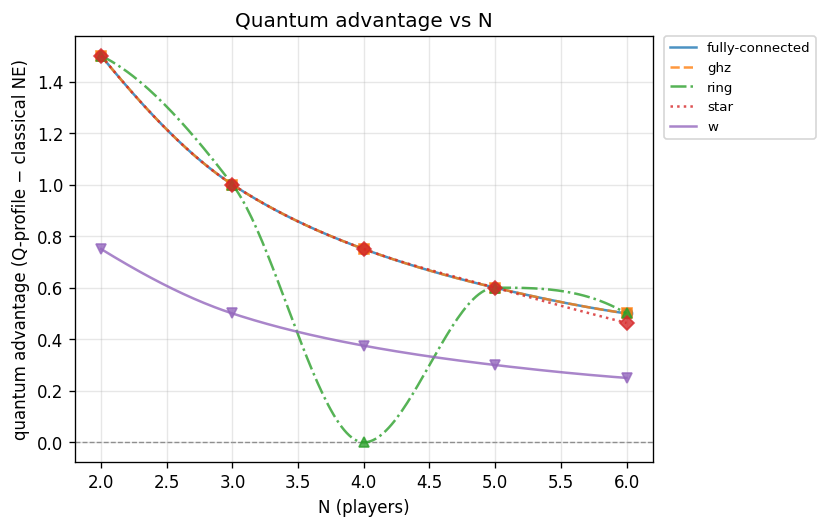
\includegraphics[width=\linewidth]{advantage_vs_N.png}
\caption{Zero-noise circuit-relative payoff gap of the fixed profile
$(Q_N,\dots,Q_N)$, defined as its mean payoff minus the highest-mean
circuit-evaluated restricted $\{D,H\}$ equilibrium payoff, at
$\gamma=\pi/2$ and $V{=}4, C{=}3$. The $3/N$ gap (star markers) is attained by
GHZ and fully connected at every recorded $N$; the ring has zero gap at
$N{=}4$; the star shows a weaker $N{=}6$ value ($0.463$ vs.\ $0.5$); and W
tracks below throughout. Filled markers indicate that the profile passes the
restricted $\{D,H,Q_N\}$ deviation check, which depends on topology.}
\label{fig:advmap}
% source: results/n-scaling-advantage/2026-07-19T0901Z/plots/advantage_vs_N.png
\end{figure}

\begin{figure}[t]
\centering
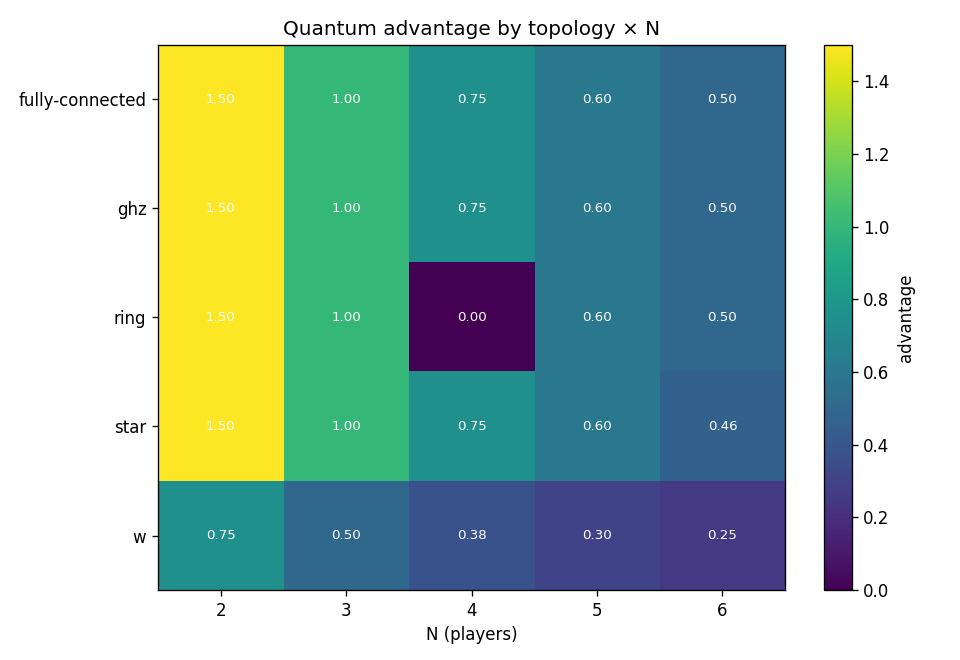
\includegraphics[width=\linewidth]{topology_heatmap.png}
\caption{Circuit-relative payoff-gap heatmap across the
$(N,\text{topology})$ grid at $V{=}4, C{=}3$ (mean per-player payoff of
$(Q_N,\dots,Q_N)$ minus the highest-mean circuit-evaluated restricted
$\{D,H\}$ equilibrium payoff). GHZ and fully connected hold the $3/N$ gap
everywhere; the single dark cell is the ring at $N{=}4$ (gap exactly $0$).}
\label{fig:heat}
% source: results/n-scaling-advantage/2026-07-19T0901Z/plots/topology_heatmap.png
\end{figure}

\subsection{Entanglement-Angle Dependence}
% gamma-sweep data: results/gamma-sweep/N2..N6 (V=4/C=3, fixed mode, noiseless)
Sweeping $\gamma$ separates a cooperative payoff gap from an
entanglement-enabled restricted-menu equilibrium. At $\gamma=0$, $J=I$ and
the phase-only $Q_N$ profile is measurement-equivalent to all-Dove: its
positive payoff gap over all-Hawk is classical in outcome probabilities and
the profile does not pass the restricted deviation check. At nonzero
$\gamma$, the same sweep records when the fixed profile begins to pass that
finite-menu check.

At $N{=}2$ every topology's circuit-relative payoff gap is positive from
$\gamma{=}0$, and $(Q,Q)$ begins to pass the restricted deviation check from
$\gamma=0.3\pi$ (W excepted, which never passes in range). At $N{=}3$ GHZ,
fully connected, and ring hold a gap of $1.0$ across the sweep and begin to
pass at $\gamma=0.3\pi$--$0.4\pi$; star and W never pass. At $N{=}4$
(Fig.~\ref{fig:gamma}) GHZ and star hold $0.75$ at every $\gamma$, fully
connected dips to $0.40$ mid-sweep and recovers, W decays monotonically to
$0.375$, and ring reaches exactly zero at $\gamma=\pi/2$, the same
$N{=}4$ interference zero. No series has a negative circuit-relative payoff
gap; only that ring endpoint reaches zero.

\begin{figure}[t]
\centering
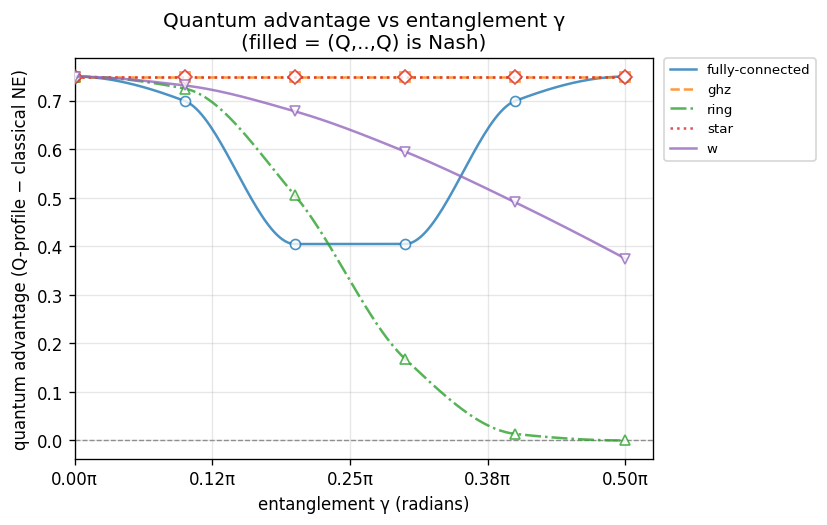
\includegraphics[width=\linewidth]{advantage_vs_gamma_N4.png}
\caption{Circuit-relative payoff gap versus entanglement angle $\gamma$ at
$N{=}4$ ($V{=}4, C{=}3$, noiseless). GHZ and star hold $0.75$ flat; fully
connected dips and recovers; W decays monotonically; and ring falls to zero at
$\gamma=\pi/2$. Data:
\texttt{results/gamma-sweep/N4}.}
\label{fig:gamma}
\end{figure}

\subsection{Player Symmetry Breaking in the Star Topology}
% star per-player data: results/n-scaling-advantage/2026-07-19T0901Z/plots/per_player_advantage_star.png
The star is the only topology that breaks player symmetry at zero noise. For
$N\ge4$ its per-player circuit-relative payoff gaps are uneven
(Fig.~\ref{fig:star}): at $N{=}4$ the three leaves have gap $1.0$ each while
the hub has $0.0$; by $N{=}6$ the hub has $0.952$ against the leaves' $0.366$.
The mean circuit-relative payoff gap stays close to $3/N$ until $N{=}6$, where
the hub--leaf split pulls it to $0.463$.

\begin{figure}[t]
\centering
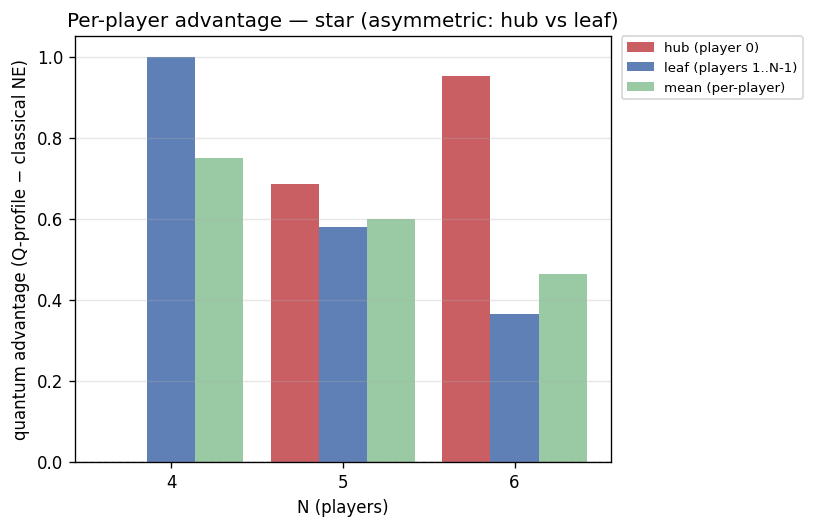
\includegraphics[width=\linewidth]{per_player_advantage_star.png}
\caption{Star-topology per-player circuit-relative payoff gap (hub player 0
vs.\ each leaf) at $\gamma=\pi/2$, $V{=}4, C{=}3$, noiseless, for
$N=2\ldots6$. The leaves capture the gap at small $N$; the hub captures it at
large $N$; the mean (dashed) tracks $3/N$ until $N{=}6$. Data:
\texttt{results/n-scaling-advantage/2026-07-19T0901Z}.}
\label{fig:star}
\end{figure}

\subsection{Noise Robustness: Two Criteria Disagree}\label{sec:noise}
% ported from README §9 (Month-4, corrected 2026-07-17); data results/noise-robustness/2026-07-03T0213Z
Sweeping the depolarizing strength $p$ from $0$ to $0.05$ on the gate-level
noisy path, two natural ``robustness'' criteria give different orderings, so
we state which we mean.

\subsubsection{Restricted-menu equilibrium criterion}
Under this criterion, the GHZ cooperative profile passes at $p=0$ only for
$N{=}2,3$, and at $N{=}3$ it loses that status between $p=0.04$ and $0.045$.
For $N{=}4,5$ the GHZ thresholds $p^*\approx0.0197$ and $0.0098$ are
\emph{circuit-relative payoff-gap zero crossings}, not equilibrium losses:
the profile does not pass the restricted deviation check there even at
$p=0$. The fixed-mode zero-noise artifact records ring as passing at
$N{=}2,3$, fully connected at $N{=}2,3$, star at $N{=}2$, and W at neither
$N{=}2$ nor $N{=}3$.

\subsubsection{Circuit-relative payoff-gap magnitude criterion}
Under this criterion the picture flips: at $N{=}3$ GHZ retains the largest
mean gap at $p=0.05$ ($0.333$, $33\%$ of its noiseless value) versus ring
$0.200$ and W $0.047$. These are not crossings relative to the analytic $1/N$
baseline: noise can change both the fixed-profile payoff and the highest-mean
restricted $\{D,H\}$ circuit equilibrium, and comparator drift can drive a
zero crossing. The natural-budget ordering therefore characterizes the
production circuits. Matched-count controls reduce gate-budget confounding
within the XX family, whose normalized per-$cx$ decay rates are similar in the
control table at approximately 1.8--2.7; no statistical equivalence test was
recorded. Absolute GHZ--W payoff-gap ordering can remain after those controls
because their zero-noise gaps differ. W is the normalized-retention outlier at
approximately $0.8$--$1.0$ per CX. It keeps a positive but small mean
circuit-relative gap across the whole grid, while the mean hides per-player
losses: at $N{=}5$ two of the five players have negative per-player gaps from
$p=0.01$ (worst $-0.077$ at $p=0.015$). All entanglers here are exact
gate-level circuits; W uses the T8 construction (44 and 68 $cx$ per $J$ at
$N{=}4,5$, versus $100$/$444$ for the retired transpiled-unitary fallback).

\subsection{Position-Locked Unfairness}
% wiring-permutation: README §9 Month-4 findings
The noise-induced per-player asymmetry is not a property of the player labels
or the ideal state. A wiring-permutation test on the ring at $N{=}5$
implemented in \texttt{scripts/}\allowbreak\texttt{asymmetry\_diagnostics.py}
cyclically shifts the
qubit-to-player wiring and the whole per-player payoff vector permutes
rigidly with it (deviation $\sim10^{-16}$); and applying the same depolarizing
weight to the \emph{ideal final state} instead of per-gate collapses the
per-player spread to $\sim0$. The disadvantage therefore follows the
entangler's \emph{circuit position} (gate ordering), not the ideal state or
the player identity.

A distinct graph-role asymmetry was tested on hardware. A registered wiring-permutation control on
the star at $N{=}4$ (Sec.~\ref{sec:hwtopology},
Fig.~\ref{fig:hwtopology}C) reassigns players to different physical qubits and
moves the measured per-player payoff vector by at most $0.035$, inside the
registered threshold, while the hub--leaf split itself
($\approx 0.34$ against $\approx 1.21$) is unchanged. The ring simulation identifies sensitivity to circuit ordering. The star
hardware control supports persistence of its hub--leaf asymmetry under the
tested physical assignments; it does not identify the cause of the ring effect.

\subsection{The Finite-Round Adaptation Pilot}
% T9 pilot: docs/findings/2026-07-05-t9-adaptation-fairness.md
An exploratory W-state pilot at $N{=}4$ tested one provisional independent
round-robin best-response rule. No tested setting produced a beneficial
converged fairness repair: at $p=0$ the dynamics reached the 50-round cap
near mean $0.51$ without converging; at $p=0.02$ they entered a payoff limit
cycle with lower mean and larger spread; and at $p=0.05$ they converged with
little change. Two robustness checks were then run on this pilot, both
simulation-only. Replacing round-robin with \emph{simultaneous} best response,
which removes move order entirely, reproduces all three verdicts, so the
$p=0.02$ non-convergence is a property of the noisy best-response map rather
than of the update order. Extending to $N{=}5$, W $N{=}5$ reproduces the
$N{=}4$ verdicts, while ring $N{=}5$ fails to converge at every noise level
tested and does so in the opposite direction: it drives a perfectly fair
$p{=}0$ baseline apart while leaving mean welfare unchanged, i.e.\ it
redistributes rather than shrinks. Because those ring endpoints are snapshots of
non-convergent trajectories we report the direction only and not the magnitudes.
Belief-based rules such as fictitious play remain untested, and the pilot
remains exploratory pending game-theory sign-off.

% =============================================================================
\subsection{Alternative Phase and Compact Evaluation}\label{sec:phase-results}
% results/journal-strengthening/2026-09-07-offline/results.json
The incentive boundary of Sec.~\ref{sec:incentive-boundary} separates a
phase-choice limitation from a player-count limitation. At $N=4,5,6,7$,
the alternative profile's minimum ideal Hawk/Dove gaps are respectively
$0.7500$, $0.4180$, $0.5000$, and $0.3734$, whereas the original profile
has a profitable Hawk deviation at each size. These are ideal results;
the historical device experiments used the original phase. New tests of
the alternative strategy are reported in Sec.~\ref{sec:phase-hardware}.
The unrestricted witness remains
profitable for both branches.

The ideal GHZ circuit also permits compact classical evaluation. Write
$c=\cos(\gamma/2)$, $s=\sin(\gamma/2)$,
$A=\bigotimes_j U_j\ket0$, and $B=\bigotimes_j U_j\ket1$.
Expanding the preparation and inverse in Eq.~\eqref{eq:ewl-state} gives
\begin{equation}
\ket{\psi_{\mathrm{out}}}
=c^2 A+isc B-isc X^{\otimes N}A+s^2 X^{\otimes N}B.
\label{eq:four-branches}
\end{equation}
Thus the output is a sum of at most four product states, even for
nonidentical local strategies, and its Schmidt rank across every
bipartition is at most four. This is a classical representation bound
for the ideal GHZ circuit, not a bound for every family or noisy implementation.

Per-player payoffs can be evaluated without enumerating outcomes using
\begin{equation}
\pi_j=\frac VN p(0^N)
+V\,\mathbb E\!\left[\frac{x_j}{k}\mathbf1_{\{k>0\}}\right]
-\frac CN p(1^N).
\label{eq:compact-payoff}
\end{equation}
For each pair of product branches, $1/k=\int_0^1z^{k-1}\,dz$ turns
the middle term into a polynomial integral of degree $N-1$.
Gauss--Legendre quadrature with $\lceil N/2\rceil$ nodes integrates it
exactly up to floating point. Prefix and suffix products evaluate all
players at each node in linear work, giving quadratic work overall.
The implementation uses no $2^N$ probability array or dense entangler.
Tests compare arbitrary-profile payoffs with the dense oracle through
$N=7$; the resource experiment extends evaluation to $N=128$.
Timings in Fig.~\ref{fig:journal-extensions} include memory instrumentation
overhead and are single-machine measurements, not asymptotic speedup evidence.
Checking a fixed three-strategy candidate needs $1+2N$ profile evaluations;
enumerating all equilibria still requires a separate search.

For a fixed profile, we also replace heuristic unilateral optimization
with a global local-unitary response calculation. Quaternion quadratic-form
methods already occur in two-player quantum-game analysis~\cite{landsburg2011};
here we use the single-gate structure with fixed multiplayer opponents. Write
$U(q)=q_0I+i(q_1X+q_2Y+q_3Z)$ with real $\|q\|=1$.
Linearity of circuit amplitudes in this single gate makes the payoff
$q^TM_jq$ for a real symmetric $4\times4$ matrix. Four coordinate
evaluations and six normalized pair sums determine $M_j$; its largest
eigenvalue is the best-response payoff and its eigenvector supplies a
witness. Independent evaluations check the reconstruction and witness.
This certifies a response to fixed opponents in the specified circuit,
not convergence of a search for an equilibrium. Strategy-dependent noisy
compilation requires separate validation of the quadratic assumption.

\subsection{Sensitivity to Partial Conflict Costs}\label{sec:payoff-sensitivity}
The mean-welfare identity implies that analytic-baseline retention equals
$1-p(1^N)$. Uniform independent classical bits therefore retain
$1-2^{-N}$, or $99.21875\%$ at $N=7$. This randomization is not an
equilibrium of the underlying dominance game; it demonstrates why high
retention alone does not establish coherent cooperation or useful
incentive compatibility. All output patterns with between one and
$N-1$ Hawks preserve the original total welfare.

We test the dependence on that payoff rule with a separate sensitivity
game. Let $\ell\in[0,1]$ and define total conflict loss
\begin{equation}
L_\ell(k)=C\left[(1-\ell)\mathbf1_{\{k=N\}}
+\ell\frac{k(k-1)}{N(N-1)}\right].
\label{eq:partial-conflict-loss}
\end{equation}
All-Dove still pays $V/N$; at $k>0$ each Hawk receives
$(V-L_\ell(k))/k$ and each Dove zero. The original game is $\ell=0$,
while $\ell=1$ charges according to the fraction of Hawk pairs. Both
endpoint payoffs and the $N=2$ game are preserved. At $V>C$, Hawk remains
strictly dominant since its payoff is positive against every nonempty
Hawk set and is $V>V/N$ against all-Dove.

We retrospectively reweight saved raw fold-1 counts at
$\ell=0,0.25,0.5,1$, without claiming new hardware execution or new
equilibrium tests. For the $N=3,\ldots,7$ extension run, retention at
$\ell=1$ is respectively $98.17\%$, $96.00\%$, $94.91\%$, $92.46\%$,
and $93.23\%$, compared with $75\%$ for uniform independent outcomes
at every size. At $N=7$ the corresponding raw player floor is $0.4993$.
Sampling intervals come from the same count distributions; they exclude
calibration drift. This sensitivity model is not an empirically fitted
economic model, and reweighting cooperative counts does not establish
its noisy equilibria.

\begin{figure*}[t]
\centering
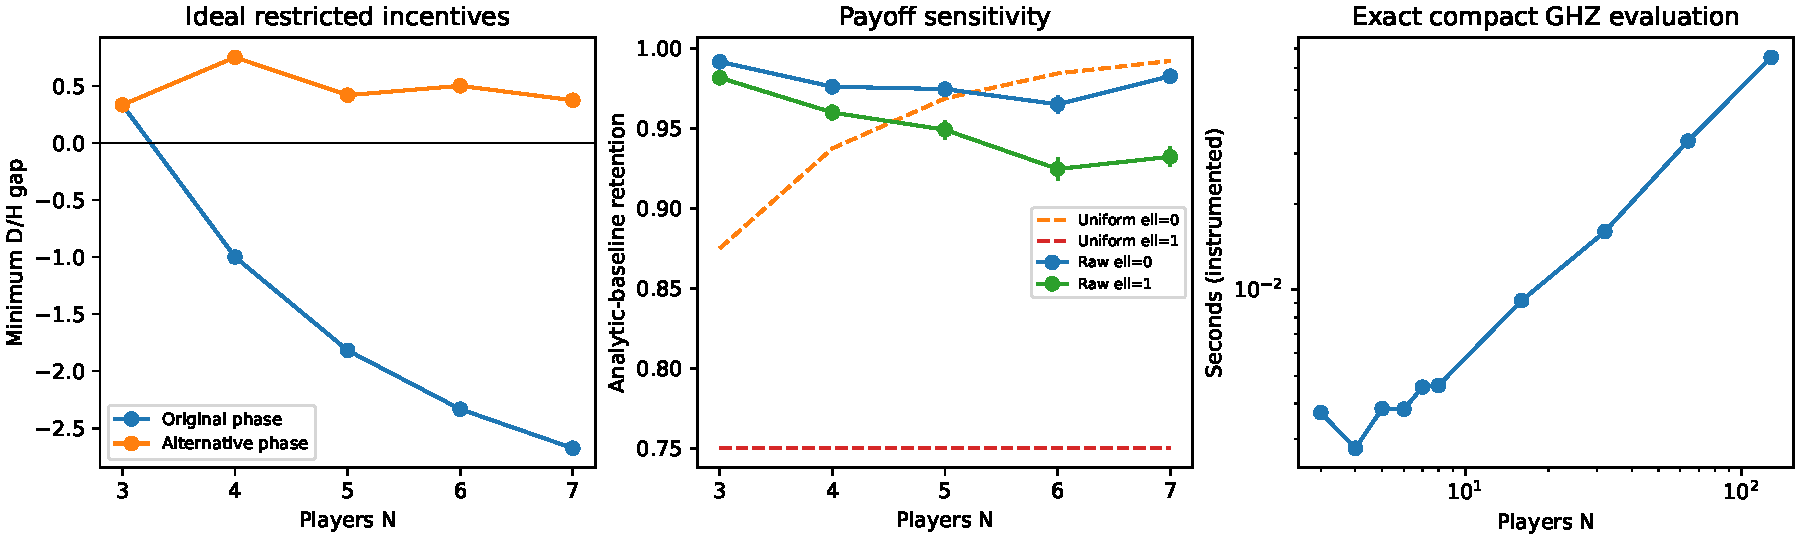
\includegraphics[width=\textwidth]{journal_extensions.pdf}
\caption{Journal-extension analyses. Left: minimum ideal Hawk/Dove deviation
gap for the original and alternative cooperative phase branches, each in its
stated restricted menu. Middle: retrospective raw fold-1 retention under the
original and partial-conflict payoff rules for the recorded $N=3$--$7$ run;
error bars are $1.96$ multinomial standard errors and exclude calibration drift.
Uniform independent-outcome comparators are diagnostic, not equilibria.
Right: exact compact GHZ payoff evaluation through $N=128$; instrumented CPU
time is a classical resource measurement, not hardware player-count scaling.}
\label{fig:journal-extensions}
\end{figure*}


\section{Hardware Validation on IBM Heron r2}\label{sec:hardware}

\subsection{Experimental Setup and Safeguards}
Every submission passes three gates: (i) an $\mathrm{Operator.equiv}$
circuit-identity assertion against the dense
$J^\dagger (U^{\otimes N}) J$ reference, (ii) a noiseless simulator dry-run
that must reproduce the exact analytic advantage, and (iii) a full dress rehearsal of the batch, including mitigation analysis, on the device
noise model reduced to the executed qubits. Job identifiers are persisted
before result polling, making runs crash-safe and recoverable. The execution
configuration common to all runs is summarised in Table~\ref{tab:hwconfig}.
% experiments/hardware_scaling.py; spec docs/superpowers/specs/2026-07-16-*.md

\begin{table}[t]
\centering
\caption{Hardware Execution Configuration}
\label{tab:hwconfig}
\footnotesize
\begin{tabular}{@{}ll@{}}
\toprule
\textbf{Parameter} & \textbf{Value}\\
\midrule
Device & ibm\_fez (IBM Heron r2)\\
Shots per circuit & 4096\\
$N{=}3$ validation chain & $[136,143,142]$\\
Scaling chain ($N{=}3,4,5$) & $[59,75,74,73,79]$\\
Extension chain ($N{=}3\ldots7$) & $[97,107,108,109,110,111,98]$\\
Readout mitigation & tensored confusion-matrix inversion\\
Zero-noise extrapolation & local cz folding, $\lambda\in\{1,3,5\}$\\
Batch sizes & 11-pub scaling, 17-pub extension,\\
 & 49-pub multi-topology\\
Software & qiskit 1.3.2 / qiskit-aer 0.14.2 /\\
 & qiskit-ibm-runtime 0.36.1\\
\bottomrule
\end{tabular}
\end{table}

\subsection{Single-Point Validation at $N=3$}
% results/hardware-n3/2026-07-16T013912Z/ (job d9br6l66hjac73fg3g7g)
We ran the validated $Q_3$ circuit (entangler decomposed to 6 native cz gates)
with 4096 shots on ibm\_fez; $3911/4096$ shots landed in $\ket{000}$
(Fig.~\ref{fig:n3}). The measured mean payoff is $1.3311$, or
$99.835\%$ of the ideal payoff $4/3$; subtracting the analytic all-Hawk
baseline $1/3$ gives measured advantage $0.9978$, or $99.780\%$ of the ideal
advantage $1.0$.

A product of the recorded readout fidelities ($0.9960$, $0.9961$, $0.9962$)
and two-qubit fidelities (edge errors $0.17\%$ and $0.23\%$, applied in the
recorded four-plus-two \textsc{cz} split) gives a heuristic ground-state
probability of about $0.977$, whereas the measured value is
$3911/4096=0.955$. Under a fixed binomial interpretation the difference is
about $9.5$ standard deviations, so the product has the right order of
magnitude but substantially underpredicts non-ground weight; it is not a
calibrated statistical model of this execution.
% run: results/hardware-n3/2026-07-16T013912Z job d9br6l66hjac73fg3g7g;
% readout_error 136/143/142, twoq_gate_error 136_143 / 143_142;
% p_naive = prod(1-r_i) * (1-g_a)^4 (1-g_b)^2 = 0.9771 (4+2)

For every outcome with $0<k<N$ Hawks, total payoff remains $V$, so the mean
remains $V/N$. Only the all-Hawk outcome lowers total payoff to $V-C$:
\begin{equation}
\overline{\pi}=\frac{V}{N}-\frac{C}{N}P(1\ldots1).
\end{equation}
In the measured counts, $176$ of the $185$ shots outside $\ket{000}$ land on
one- and two-Hawk outcomes, while only the $9$ all-Hawk shots ($0.22\%$) lower
the mean. The identity reconstructs the measured payoff $1.3311$ and advantage
$0.9978$.
% counts: k=0:3911, k=1:53, k=2:123, k=3:9 (result.json counts block)
The mean-payoff observable is therefore first-order insensitive to single
bit-flips from the ideal outcome: errors that flip one qubit redistribute
payoff between players without lowering its mean. This is the structural
mechanism behind the scaling section's central observation, that the advantage decays several times slower than the all-zero target-state population, and it is why the
$N{=}3$ advantage survives at $99.780\%$ of its ideal while
$P(\ket{000})$ has already lost $4.5\%$.

\begin{figure}[t]
  \centering
  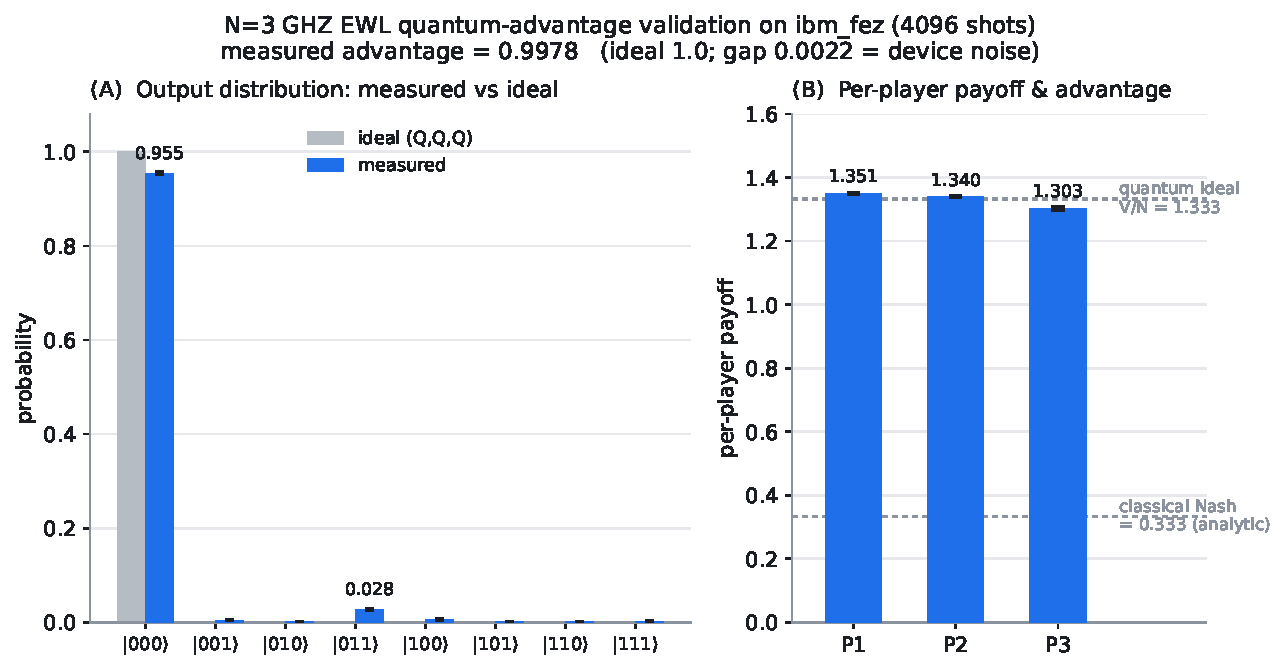
\includegraphics[width=\linewidth]{hardware_n3_validation.pdf}
  \caption{Hardware validation of the $N{=}3$ GHZ EWL quantum advantage on
  ibm\_fez (IBM Heron r2). The validated $(Q,Q,Q)$ circuit, with entangler $J$ decomposed to 6 native cz gates, was executed with 4096 shots.
  \textbf{(A)} Measured output distribution over the eight
  computational-basis states (blue) versus the noiseless ideal (grey); error
  bars are binomial shot noise. $3911/4096$ shots (95.5\%) fall in
  $|0\ldots0\rangle$, the ideal $(Q,Q,Q)$ output. \textbf{(B)} Measured
  per-player payoff (blue) against the analytic classical-Nash baseline
  ($0.333$, noiseless) and the quantum ideal $V/N=1.333$; error bars
  propagate shot noise. The measured mean payoff $1.331$ gives advantage
  $0.9978$ vs the ideal $1.0$. Physical qubits $\{136,143,142\}$ (calibration
  2026-07-15): readout error 0.38--0.40\%, cz error 136--143: 0.17\%,
  143--142: 0.23\%.}
  \label{fig:n3}
\end{figure}

\subsection{Scaling at $N=3,4,5$ with Error Mitigation}
% results/hardware-scaling/2026-07-16T074134Z/ (job d9c8fpn550hc73dl1tcg)
All three $N$ ran on prefixes of one pinned 5-qubit chain
$[59,75,74,73,79]$ (chosen by calibration error) in a single 11-pub batch:
two readout-calibration circuits plus $N\in\{3,4,5\}\times$ cz-fold
$\lambda\in\{1,3,5\}$. Readout errors are corrected by tensored confusion-matrix
inversion (constrained least squares)~\cite{maciejewski2020,bravyi2021pra}; zero-noise
extrapolation folds each cz locally ($\mathrm{cz}\to\mathrm{cz}^\lambda$,
unitary-preserving since cz is self-inverse) and extrapolates the
readout-mitigated payoff linearly to $\lambda=0$~\cite{temme2017,kandala2019}.

\begin{table}[t]
\centering
\caption{Measured advantage on ibm\_fez for the registration-source execution
(4096 shots). Repeat executions are discussed separately; the cross-calibration
aggregate over both epochs is Fig.~\ref{fig:scaling}. Ideal advantage is $3/N$;
retention is ZNE/ideal.}
\label{tab:scaling}
\begin{tabular}{@{}ccccc c@{}}
\toprule
$N$ & ideal & raw & mitig.+ZNE & retention & $P(\ket{0\ldots0})$\\
\midrule
3 & 1.00 & 0.9919 & 0.9938 & 99.4\% & 0.938\\
4 & 0.75 & 0.7386 & 0.7403 & 98.7\% & 0.922\\
5 & 0.60 & 0.5837 & 0.5887 & 98.1\% & 0.868\\
\bottomrule
\end{tabular}
\end{table}

\begin{figure*}[t]
  \centering
  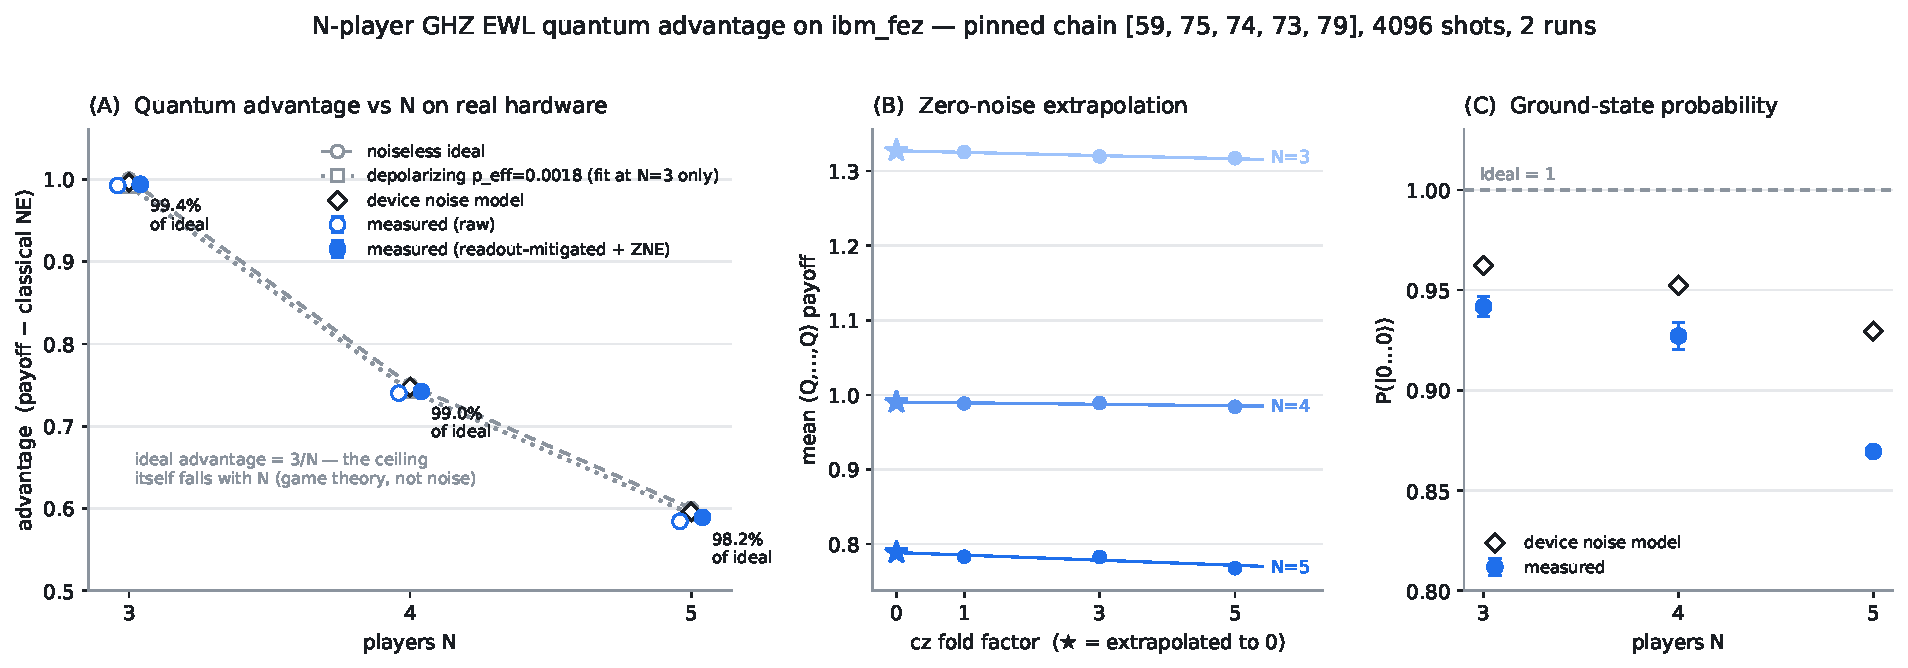
\includegraphics[width=\textwidth]{hardware_scaling.pdf}
  \caption{Cross-calibration aggregate of the $N$-player GHZ EWL quantum
  advantage on ibm\_fez (IBM Heron r2): three executions spanning
  \emph{two distinct provider calibrations}, all on the same physical chain
  $[59,75,74,73,79]$, 4096 shots each. Executions sharing a calibration stamp
  are averaged into one point before the spread is taken, because two runs
  under one calibration are one sample rather than two; the two epochs are
  2026-07-16 08:30:13 (two executions) and 2026-07-26 13:29:01 (one).
  A fourth execution exists on chain $[20,21,22,23,24]$ and is deliberately
  \emph{excluded} here: pooling it would confound calibration drift with a
  change of physical qubits. Table~\ref{tab:scaling} reports the
  registration-source execution alone.
  \textbf{(A)} Measured cooperative-profile advantage (mean $(Q,\ldots,Q)$
  payoff minus the analytic noiseless classical-Nash payoff) at $N=3,4,5$:
  raw (open) and readout-mitigated $+$ ZNE (filled), against the noiseless
  ideal ($1.0, 0.75, 0.6$), the device noise-model prediction (diamonds), and
  a single-parameter depolarizing model with $p_{\mathrm{eff}}=0.0018$ fitted
  to the $N{=}3$ point alone; its $N{=}4,5$ values are predictions, not fits. The ideal, device-model and depolarizing curves are the
  registration anchor's rather than run averages, so the registered
  $p_{\mathrm{eff}}$ is quoted unchanged. Error bars are the sample standard
  deviation across the two calibration epochs, a genuine cross-calibration estimate unlike the within-epoch spread reported in earlier drafts, and still exclude the within-run multinomial and weighted-fit standard errors,
  so they are a lower bound on total uncertainty. \textbf{(B)} ZNE mechanics:
  readout-mitigated payoff vs cz
  fold factor ($\lambda=1,3,5$) with the weighted linear fit extrapolated to
  $\lambda=0$ (stars). \textbf{(C)} Ground-state probability
  $P(|0\ldots0\rangle)$: the all-zero target-state population decays several times faster than
  the advantage because the mean-payoff observable is first-order insensitive
  to single bit-flips from $|0\ldots0\rangle$. $(Q,\ldots,Q)$ passes the
  restricted-menu pure-Nash check only at $N{=}3$ among the plotted genuinely
  multiplayer cases; at $N{=}4,5$ the profile is the cooperative quantum
  protocol, not an equilibrium.}
  \label{fig:scaling}
\end{figure*}
% aggregate source: results/hardware-scaling/2026-07-26T090122Z/plots/hardware_scaling.pdf
% (+ caption.md there records the epoch grouping and the two exclusions verbatim)
% cross-epoch ZNE advantage, per epoch:
%   2026-07-16 08:30:13  N=3 0.9938  N=4 0.7422  N=5 0.5892
%   2026-07-26 13:29:01  N=3 0.9944  N=4 0.7357  N=5 0.5811
% aggregate: N=3 0.9941+-0.0004, N=4 0.7389+-0.0046, N=5 0.5852+-0.0057

Two model predictions frame Table~\ref{tab:scaling}: the reduced device noise
model (\texttt{NoiseModel.from\_backend}) and a \emph{fit-one-predict-two}
test in the paper's own depolarizing model, with a single
$p_{\mathrm{eff}}=0.0018$ fitted to the $N{=}3$ mitigated-fold-1 point.
For the registration-source execution, the registered primary
mitigated-fold-1 endpoint misses at $N=4$ by $0.0043$ ($2.14\sigma$) and at
$N=5$ by $0.0101$ ($5.17\sigma$). These source-run residuals are
retrospective because the registration was written after that execution.
For the displayed ZNE endpoint, the corresponding misses are $0.0041$
($2.07\sigma$) and $0.0060$ ($3.05\sigma$). The second execution is the
prospective registered repeat: its conditional $N=4$ endpoint passes and
its $N=5$ endpoint misses by $0.0092$ ($4.74\sigma$). The repeated deficit
sign is observational, not a registered sign test.

The CZ-exponential baseline carries the smallest mean $|z|$ (the best score) of the five registered candidates in all four executions, including both
cross-calibration repeats. It nevertheless
misses $N=5$ outside the shared 95\% comparison yardstick in every run; that
yardstick is for ranking, not a model-specific calibrated interval.
\textbf{That ranking is specific to $N\le 5$}: in the registered $N=6,7$
extension (Sec.~\ref{sec:n67}) the CZ-exponential law loses to the depolarizing
model at $N{=}7$ and both fail their registered tests, so the ranking is not a
physical scaling law and does not extrapolate.
The registered target of three to five distinct calibrations is now met at
three, and the $N=5$ deficit reproduces with the same sign in all three
repeats. The deficit magnitude is not stable across epochs, however: it ranges
from $0.0092$ to $0.0186$, so the epoch-to-epoch variation is itself of order
the effect. Model-specific predictive uncertainties remain needed, and the
cross-calibration sample that is chain-matched is two epochs rather than three.
% registered: results/hardware-scaling/preregistration.json and
% preregistration-baselines.json; outcomes:
% results/hardware-scaling/repeat-judgments.json
% (run 1: cz 10.0 vs p_eff 31.3; run 2: cz 7.4 vs p_eff 23.4)

\subsection{Extension to $N=6,7$}\label{sec:n67}
% results/hardware-scaling/2026-07-25T180549Z/ (job d9if010gk0ls73f4avkg)
% registered: results/hardware-scaling/preregistration-n67.json (commit 8d1e5d1)
% judged: results/hardware-scaling/2026-07-25T180549Z/judgments-n67.json
% finding: docs/findings/2026-07-25-scaling-n67-run1.md
A later execution extends the curve to $N=3,\ldots,7$ on one pinned seven-qubit
chain $[97,107,108,109,110,111,98]$ (17 pubs, 20 QPU-seconds). The chain was
written into the registration and held at submission, so the executed qubits
provably match the ones the predictions describe. Measured mitigated fold-1
advantage retains $99.2\%$, $97.5\%$, $97.3\%$, $96.3\%$ and $98.1\%$ of the
ideal $3/N$ at $N=3,\ldots,7$ while $P(\ket{0\ldots0})$ falls from $0.943$ to
$0.784$: \textbf{the advantage survives to seven players at $98\%$ of ideal
with the all-zero target-state population already down to $0.78$}, which is the
first-order-insensitivity mechanism operating across the full curve.

Two competing one-parameter models were registered before submission, both
fitted on the same $N{=}3$ point and extrapolated with no $N>3$ information: the
depolarizing $p_{\mathrm{eff}}$ model and the CZ-exponential retention law
$A_N = A^{\mathrm{ideal}}_N r^{\,\mathrm{cz}_N}$. \emph{Both failed the
registered $1.96\sigma$ test at $N=6,7$}, and they failed differently: the
depolarizing model over-predicts at every $N$, while the CZ-exponential model
over-predicts at $N=4,5,6$ and then under-predicts at $N=7$. A one-parameter
retention law fitted at $N{=}3$ cannot reproduce that curvature.

The registered model race also split: the CZ-exponential law is closer at
$N=4,5,6$ but the depolarizing model is closer at $N=7$. \textbf{The
CZ-exponential ranking reported below therefore does not extrapolate past
$N{=}5$}, and we scope it accordingly. Finally, measured advantage is strictly
decreasing in $N$ (the registered monotonicity check), but \emph{retention} is
not: $N{=}7$ keeps more of its ideal advantage than $N=4,5,6$ despite carrying
the most gates and the lowest target-state population, and its ZNE estimate overshoots the
noiseless ideal ($0.4437$ against $0.4286$), which no physical noise model can
produce. We report this as an unexplained observation rather than a result.
Distinguishing payoff geometry at odd $N$ from an end-of-chain qubit effect or
an extrapolation artefact requires a repeat \emph{of this $N=3\ldots7$ batch
specifically}: the cross-calibration repeats aggregated in
Fig.~\ref{fig:scaling} re-execute the registered $N=3,4,5$ batch and so cannot
address it, and no such $N=6,7$ repeat has been run.

\subsection{Topology, Equilibrium and Fairness on Device}\label{sec:hwtopology}
% results/hardware-topology/2026-07-25T114621Z/ (job d9ia1pd0k0jc738jaqgg)
% registered: results/hardware-topology/preregistration.json (commit 46f43d4)
% judged: .../judgments.json; finding: docs/findings/2026-07-25-topology-hardware-run1.md
The experiments above are all GHZ. To put the paper's topology, equilibrium and
fairness claims on device data we ran a single 49-pub batch (4096 shots,
55 QPU-seconds) spanning five entangler topologies, unilateral strategy
deviations, wiring permutations and an entanglement-angle sweep, with all
predictions registered before submission. Cells were selected from
\emph{measured} routed \textsc{cz} counts on the real coupling map rather than
from pre-routing gate counts: on heavy-hex hardware the two differ sharply, and
fully-connected $N{=}5$ ($67$ \textsc{cz}) and W $N{=}4,5$ ($107$, $219$) were
excluded on that basis.

\begin{table}[t]
\centering
\caption{Multi-topology batch on ibm\_fez (job \texttt{d9ia1pd0k0jc738jaqgg},
4096 shots, one pinned qubit set). Retention is measured mitigated fold-1
advantage as a fraction of \emph{that cell's own} noiseless advantage, which is
not $3/N$ for every topology.}
\label{tab:topology}
\begin{tabular}{@{}lccccc@{}}
\toprule
topology & $N$ & cz & ideal adv & measured & retention\\
\midrule
GHZ             & 3 &  6 & 1.0000 & 0.9886 & 98.9\%\\
GHZ             & 4 &  9 & 0.7500 & 0.7425 & 99.0\%\\
GHZ             & 5 & 14 & 0.6000 & 0.5921 & 98.7\%\\
ring            & 3 & 10 & 1.0000 & 0.9899 & 99.0\%\\
ring            & 4 & 20 & 0.0000 & 0.0894 & n/a\\
ring            & 5 & 28 & 0.6000 & 0.5960 & 99.3\%\\
star            & 3 &  5 & 1.0000 & 0.9934 & 99.3\%\\
star            & 4 &  9 & 0.7500 & 0.7423 & 99.0\%\\
star            & 5 & 17 & 0.6000 & 0.5977 & 99.6\%\\
fully-conn.     & 3 & 10 & 1.0000 & 0.9887 & 98.9\%\\
fully-conn.     & 4 & 31 & 0.7500 & 0.7389 & 98.5\%\\
W               & 3 & 42 & 1.0000 & 0.9792 & 97.9\%\\
\bottomrule
\end{tabular}
\end{table}

\begin{figure*}[t]
  \centering
  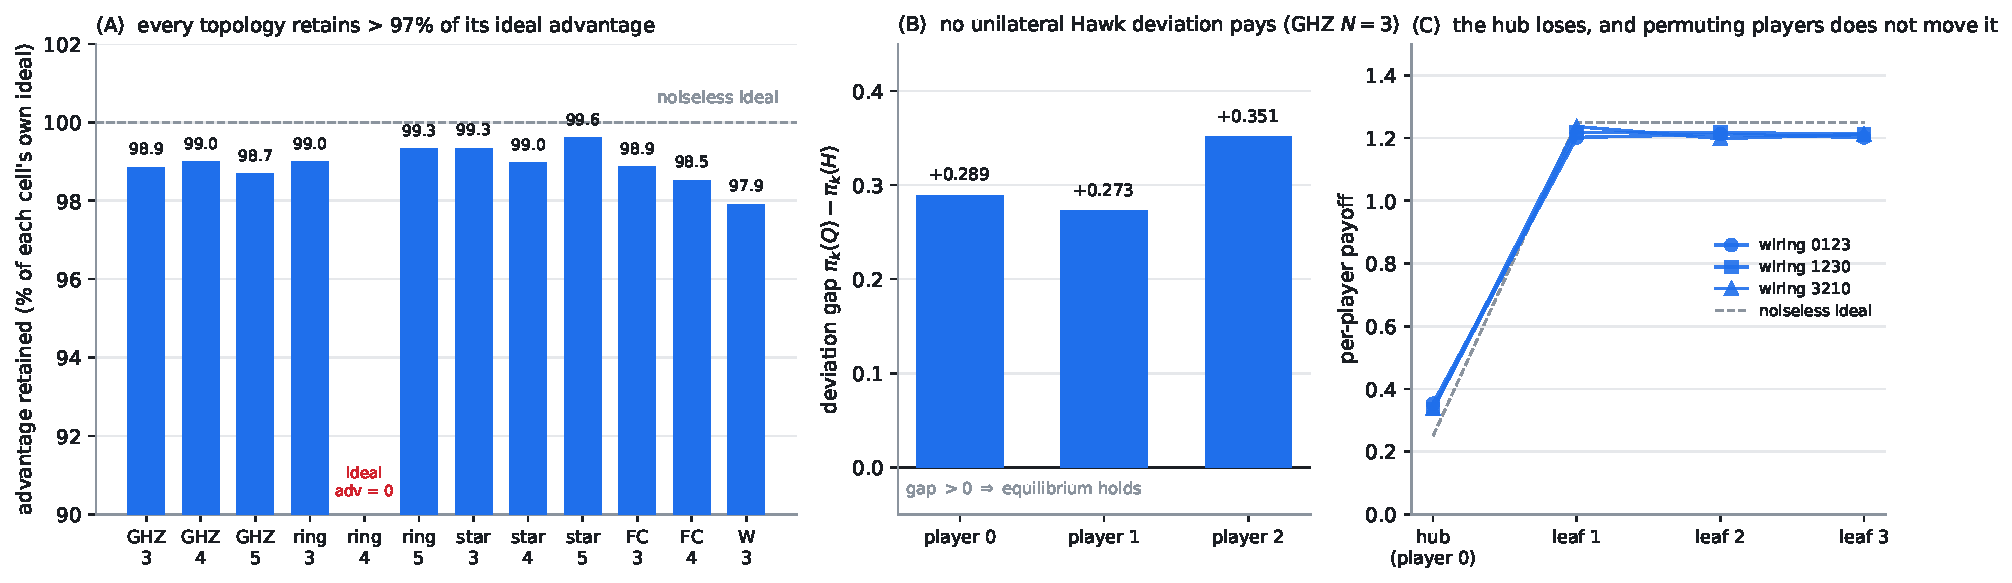
\includegraphics[width=\textwidth]{hardware_topology.pdf}
  \caption{Multi-topology EWL batch on ibm\_fez (job
  \texttt{d9ia1pd0k0jc738jaqgg}), 49 pubs $\times$ 4096 shots on one pinned
  qubit set, all predictions registered before submission.
  \textbf{(A)} Measured mitigated fold-1 advantage as a percentage of each
  cell's \emph{own} noiseless advantage; the eleven nonzero-baseline cells retain $97.9$--$99.6\%$.
  ring $N{=}4$ carries no percentage because its noiseless advantage is exactly zero: its ideal circuit is deterministic on $\ket{1\ldots1}$, so the
  $+0.089$ it measures is created by decoherence, and zero-noise extrapolation
  correctly pulls it back toward zero ($+0.037$).
  \textbf{(B)} Unilateral Hawk deviation gaps
  $\pi_k(Q,Q,Q)-\pi_k(H\text{ at }k)$ at GHZ $N{=}3$: all three are positive,
  so no measured Hawk deviation pays; Dove deviations were not measured.
  \textbf{(C)} star $N{=}4$ per-player payoffs under three wirings. The hub
  earns $\approx 0.34$ while each leaf earns $\approx 1.21$, and permuting
  players across physical qubits does not move the pattern: the disadvantage is
  locked to the graph position, not to the qubit.}
  \label{fig:hwtopology}
\end{figure*}

The eleven cells with nonzero ideal advantage retain $97.9$--$99.6\%$ of that value
(Table~\ref{tab:topology}, Fig.~\ref{fig:hwtopology}A), including W $N{=}3$ at $42$ \textsc{cz}, seven times the gate count of GHZ $N{=}3$. The
mechanism therefore is not a GHZ artefact: ring $N{=}5$ and star $N{=}5$ sit at
$P(\ket{0\ldots0}) \approx 0.10$--$0.11$, while retaining over $99\%$ of their analytic-baseline advantage.
Their ideal outputs are not generally all-zero, so these populations alone
do not measure preparation error or fidelity to their own ideal states. The
topology axis does not separate these systems by how much advantage they retain;
it separates them by \emph{structure}, as the next two results show.

\subsubsection{Registered Hawk-deviation tests on hardware}
At GHZ $N{=}3$ the three unilateral Hawk deviation gaps measure $+0.2895$,
$+0.2726$ and $+0.3512$ (Fig.~\ref{fig:hwtopology}B), all positive and many
standard errors clear of zero. This was a registered test and it passed at every
deviating position: the $(Q,Q,Q)$ profile resists the three measured Hawk deviations.
The hardware experiment does not include Dove deviations, so it does not
certify the complete $\{D,H,Q_N\}$ menu under noise. It remains
\emph{not} a full-SU(2) equilibrium claim.

A registered sweep of the same gap in the entanglement angle changes sign as
predicted: $-0.6877$ at $\gamma=0.30\pi$ and $+0.2467$ at $\gamma=0.45\pi$. The
intermediate point $\gamma=0.40\pi$ was registered in advance as marginal and
excluded from the pass criterion; it returned $+0.0067$, statistically
indistinguishable from zero. The measured Hawk-deviation incentive therefore changes sign with entanglement strength, with the
transition bracketed near $\gamma=0.4\pi$ at $N{=}3$.

\subsubsection{Position-locked unfairness is a property of the topology}
star $N{=}4$ is maximally unequal even noiselessly: the analytic per-player
vector is $(0.25,1.25,1.25,1.25)$, the hub being the loser. On device the
measured vector is $(0.353,1.202,1.212,1.202)$, and under two wiring
permutations that reassign players to different physical qubits it moves by at
most $0.035$ (Fig.~\ref{fig:hwtopology}C), inside the registered threshold.
The registered null therefore holds: \textbf{the disadvantaged position is
determined by the entanglement topology, not by which physical qubit a player
was allocated}. This supports the star graph-role effect under the tested assignments, separately from noise-induced ring circuit-order asymmetry.

\subsubsection{A cell whose advantage is made of noise}
ring $N{=}4$ is the one cell whose noiseless circuit is deterministic on $\ket{1\ldots1}$, the all-Hawk outcome, so its ideal advantage is exactly
zero. It measured $+0.089$, the smallest of the twelve cells but clearly
positive, and zero-noise extrapolation pulled it back to $+0.037$. All three
parts of that were registered in advance. A pipeline that merely inflated
whatever it touched could not produce a cell where decoherence \emph{creates}
apparent advantage and the extrapolation correctly removes it.

\subsubsection{What did not work}
The registered per-cell predictions of \emph{absolute} advantage failed, in
both the raw device-noise-model form and a CZ-linear bias-corrected form, and
that comparison is additionally confounded: the provider recalibrated between
registration and submission and the qubit selector moved the pinned set, so
those $z$-scores mix model error with a change of qubits. The five results
above are unaffected because each is a within-job differential: a payoff difference between two profiles measured on the same qubits in the same job, a
permutation against its own twin, or one cell ranked against the other eleven.
Absolute-magnitude prediction of NISQ payoffs from a device noise model remains
out of reach here; the structural claims do not depend on it.

\subsection{Why the Advantage Outlives the State}\label{sec:outlives}
Target-state population decays several times faster than the advantage
(Table~\ref{tab:scaling}): a single bit-flip from $\ket{0\ldots0}$ yields a
one-Hawk outcome whose \emph{mean} payoff is still exactly $V/N$, so the
mean-payoff observable is first-order insensitive to uncorrelated single
flips. Readout mitigation consequently moves the mean very little; its
per-player effects are mixed and remain diagnostic analyses rather than
preregistered acceptance tests. The displayed ZNE estimates are higher for
every series, but no recorded population analysis attributes that shift
specifically to suppression of CZ-created all-Hawk weight. The structural
robustness is a property of the game's payoff geometry, not of the device.

The same single-flip terms that leave the mean invariant are what create
winners and losers. Under the all-Dove branch each one-Hawk outcome transfers
$V$ to a single player and zero to the rest: the mean is protected, the
individual player is not, and under gate-level noise the disadvantaged
position is locked to the entangler's circuit layout rather than to any
coordination failure (Sec.~\ref{sec:noise}).
% docs/findings/2026-07-05-t9-adaptation-fairness.md; ring N=5 permutation
% test scripts/asymmetry_diagnostics.py (README \S9 Month-4 findings)
% simultaneous-rule check: docs/findings/2026-07-26-t9-rule-sensitivity.md
%   results/t9-pilot/precise-2026-07-26T08{44Z-p0,38Z-p0.02,25Z-p0.05}-simul
% N=5 extension: docs/findings/2026-07-26-t9-caveat2-n5-ring.md
%   results/t9-pilot/precise-2026-07-26T0904Z-w5-p0    (0.8000 -> 0.4107)
%   results/t9-pilot/precise-2026-07-26T0952Z-w5-p0.02, 0908Z-w5-p0.05
%   results/t9-pilot/precise-2026-07-26T0916Z-ring5-p0 (mean conserved 0.800000,
%     spread 0.0000 -> 1.3329 at the 50-round cap; snapshot, not a fixed point)
%   results/t9-pilot/precise-2026-07-26T09{27Z-ring5-p0.02,28Z-ring5-p0.05}
In the single exploratory W-state $N{=}4$ finite-round pilot, the provisional
independent round-robin best-response rule produced no beneficial converged
fairness repair in any tested setting. At $p{=}0$ the dynamics reached the
50-round cap near mean $0.51$ without converging; at $p{=}0.02$ they entered a
payoff limit cycle with lower mean and larger spread; and at $p{=}0.05$ they
converged with little change. The verdict survives both checks we applied to it:
it is unchanged under simultaneous rather than round-robin updates, and W
$N{=}5$ reproduces it. Ring $N{=}5$ does not converge at any noise level tested
and fails in the opposite direction, spreading a perfectly fair baseline apart
at unchanged mean welfare, reported as a direction rather than a magnitude, since those endpoints are non-convergent snapshots. No belief-based rule has been
tested. The advantage we
report can therefore coexist with unequal per-player outcomes; the per-player
floor is a relevant diagnostic for mechanism design.

\subsection{Registered Alternative-Phase Deviation Tests}
\label{sec:phase-hardware}
The new experiment evaluates $Q_N^\star$ separately from the historical
phase. On 7 September 2026, a committed registration fixed a seven-qubit
chain, $[141,142,143,144,145,146,147]$, on \texttt{ibm\_fez} and used its
prefixes for $N=3,\ldots,7$. An 18-circuit pilot preceded the complete
70-circuit batch. The complete batch contains a cooperative profile at
each size, both Hawk and Dove deviations for every player, original-phase
controls, an unrestricted counterstrategy, and two readout calibrations.
Every circuit uses 4096 shots. Dense operator identity and compiled ideal
output checks precede device-noise rehearsals and submission. The manifest
and serialized circuits are committed before each experiment, and the
execution code checks the manifest against the committed bytes.

The primary analysis uses raw implemented payoffs: calibration circuits
are diagnostic and no readout correction or ZNE is applied to these tests.
With $M=50$ primary deviations and $\alpha=0.05$, the simultaneous lower
bound on each cooperative-minus-deviation gap is
\begin{equation}
g_j^{\rm L}(a)=\widehat g_j(a)
-\sum_{s\in\{\mathrm{coop},\mathrm{dev}\}}
V\sqrt{\frac{\log(2M/\alpha)}{2n_s}},
\end{equation}
where $n_s=4096$. Hoeffding's inequality and a union bound cover the two
one-sided mean errors for every gap. These bounds assume independent
shots from stationary circuit distributions; they do not cover temporal
drift. The registered approximate-equilibrium tolerance is
$-g_j^{\rm L}(a)/(V/N)\le0.05$ for every deviation of every player.
The overall registration requires all five sizes to pass.

In the first complete batch, every measured gap is positive, but the
simultaneous criterion passes only at $N=3,4,5,6$. The minimum observed
gaps are $0.2360$, $0.5677$, $0.2157$, $0.2627$, and $0.0109$,
respectively. The corresponding maximum upper bounds on normalized
deviation gain are $0.0058$, $-0.3240$, $0.0349$, $-0.0285$, and
$0.4074$. Thus the overall registered test fails: a positive point gap
at $N=7$ does not establish the requested tolerance. At $N=4,6$ the
simultaneous lower gaps are strictly positive; at $N=3,5$ the supported
statement is approximate equilibrium at the declared tolerance.

This all-player test locates an implementation boundary absent from mean
welfare alone. At $N=7$, target population is $0.7495$ and analytic-baseline
retention is $0.9600$, despite unresolved incentive compatibility. The
experiment certifies neither arbitrary SU(2) deviations nor an enlarged
menu containing both phase families. Original-phase controls and the
unrestricted witness are separately reported diagnostics. The witness's
observed gain over cooperation for player zero ranges from $2.4604$ to
$2.7052$ across the five sizes, consistent in direction with the analytic
counterexample. These diagnostic point estimates do not enlarge the
registered finite-menu certification scope.

A second complete batch reused the frozen circuits, shots and decision rule
after a replication plan was committed. Each batch is judged separately;
their counts are not pooled to rescue a failed criterion. The repeat
supports the criterion at $N=4,6$, but not at $N=3,5,7$
(Table~\ref{tab:phase-repeat}). All 50 point gaps are positive in the first
batch; one is slightly negative in the repeat, at $N=7$. This is not a
statistically established profitable deviation. Both batches fail the
overall five-size test, while the positive lower gaps at $N=4,6$ reproduce.
The executions occurred minutes apart on the same chain; this is a
within-session repetition, not evidence across independent calibration
epochs. The pilot and two complete batches consumed $21+77+77=175$ seconds
of provider-reported charged QPU time.

\begin{table}[t]
\centering
\caption{Alternative-phase all-player tests, judged separately in each
batch. $g_{\min}$ is the smallest observed payoff gap; $u_{\max}$ is the
largest simultaneous upper bound on deviation gain normalized by $V/N$.
The registered tolerance requires $u_{\max}\le0.05$.}
\label{tab:phase-repeat}
\begin{tabular}{crrrr}
\toprule
& \multicolumn{2}{c}{First batch} & \multicolumn{2}{c}{Repeat}\\
$N$ & $g_{\min}$ & $u_{\max}$ & $g_{\min}$ & $u_{\max}$\\
\midrule
3 & 0.2360 & 0.0058 & 0.1362 & 0.0806\\
4 & 0.5677 & -0.3240 & 0.5716 & -0.3279\\
5 & 0.2157 & 0.0349 & 0.1861 & 0.0719\\
6 & 0.2627 & -0.0285 & 0.2483 & -0.0069\\
7 & 0.0109 & 0.4074 & -0.0033 & 0.4322\\
\bottomrule
\end{tabular}
\end{table}


\subsection{Scalability and Practicality}
Scalability has distinct mathematical, computational, and physical meanings
in this protocol. The alternative phase branch has an ideal restricted-menu
equilibrium for every $N$, and compact GHZ evaluation reaches $N=128$
without dense state enumeration. Neither result increases the number of
simultaneous players demonstrated on hardware: the native device evidence
ends at $N=7$. The new alternative-phase batch tests every D/H deviation
but does not resolve the registered tolerance at $N=7$. Ideal per-player gains
scale as $C/N$, incentive margins decrease with $N$, and the permitted
entanglement-angle interval narrows. Practical scaling therefore requires
explicit statistical precision and implementation budgets.

The protocol assumes a shared preparation stage and joint inverse/readout.
Our centralized experiments do not demonstrate a distributed quantum market
or remove the need to trust preparation, decoding, and enforcement of a
permitted strategy menu. Market architectures motivate interpretations of
the graph families, but are not validated deployment models. Comparisons
with classical mechanisms must state which mediation and enforcement
resources are available~\cite{vanenk2002classical}.

\subsection{Limitations and Future Work}
Our primary game fixes $V=4$ and $C=3$ in a strict-dominance regime and charges
conflict cost only at the all-Hawk outcome. High mean retention is therefore
compatible with random outcomes, unequal allocations, and profitable
deviations. The partial-conflict sensitivity analysis tests this modeling
choice retrospectively; it does not establish a realistic economic payoff
model or a noisy equilibrium of the altered game.

All restricted equilibria refer to explicitly named menus. Both cooperative
phase families admit a profitable unrestricted SU(2) deviation. Historical
device measurements tested Hawk deviations only, and do not establish
resistance to Dove deviations under hardware noise. Arbitrary quantum
channels, ancillary systems, coalitions, and adaptive multi-round strategies
are outside our certification scope. Symmetric strategy search also does not
exclude better asymmetric profiles or other equilibria.

Entangler-family comparisons depend on the chosen generator, interpolation
angle, compiled circuit, routing, and noise placement. The W results concern
one specified operator; equal nominal angles do not equalize interaction
budget or entangling power. The normalized interaction convention defined
above remains an unexecuted sensitivity control. Noiseless star graph-role
asymmetry and noise-induced ring circuit-order asymmetry are distinct effects;
the star wiring experiment alone does not identify the ring's mechanism.

Depolarizing noise is a controlled model rather than a complete device
description. Readout correction and zero-noise extrapolation introduce
assumptions and uncertainty; extrapolated estimates can exceed physical
payoff bounds. Chain-matched scaling uncertainty rests on two calibration
epochs, and the original $N=6,7$ batch has not been repeated. Registered
one-parameter models did not extrapolate reliably. The new complete
alternative-phase batches are repetitions within one session, and fail
their overall five-size criterion; only $N=4,6$ pass in both. The compact simulation
results do not extend the demonstrated physical player count. The
finite-round adaptation pilot remains exploratory and does not establish
convergence of general learning rules.


\section{Technical Differentiation}\label{sec:novelty}
Prior multiplayer EWL studies and trading experiments establish the setting
in which this work belongs~\cite{benjamin2001,chappell2012,khan2025,varsamis2025}.
Our contribution is the joint accounting of restricted incentives, payoff
geometry, and implementation-dependent fairness in a specified allocation
game. The phase-branch boundary explains why the historical cooperative
strategy fails beyond three players and provides a different ideal
restricted-menu profile, accompanied by an unrestricted counterexample.

Matched compilation controls restrict how much of a measured family ordering
can be attributed to ideal correlation structure. The payoff sensitivity
analysis likewise restricts how much high mean retention establishes about
cooperation. The registered hardware record contains both positive differential
tests and unsuccessful quantitative predictions. These components support
a study of incentive and observable robustness; they do not establish
computational quantum speedup or an operational quantum market.

\section{Conclusion}\label{sec:conclusion}
We studied how entangler family, implementation noise, and player count
affect welfare and incentives in a multiplayer EWL allocation game. The
original GHZ cooperative phase has a restricted-menu equilibrium only at
$N=2,3$, while a separately defined phase branch satisfies the ideal
restricted condition for every $N\ge2$ at maximal entanglement. Both
profiles admit an explicit profitable unrestricted SU(2) deviation.
An all-$N$ restricted existence statement therefore coexists with an
exact strategy-access limitation.

Historical hardware experiments validate the original cooperative protocol
through seven players and its resistance to measured Hawk deviations at
$N=3$. Two new complete alternative-phase batches support the registered
incentive criterion at $N=4,6$ in both runs. The $N=3,5$ criterion passes
only in the first batch, and $N=7$ remains unresolved despite high mean
retention. Both batches fail the overall registered five-size test.
High mean retention is partly built into the
all-Hawk-only conflict penalty; the uniform comparator and retrospective
partial-conflict sensitivity make that dependence explicit. At $N=7$,
the partial-conflict model retains $93.23\%$ in raw data against a $75\%$
uniform comparator, without implying an equilibrium or a computational advantage.

Compact classical evaluation through $N=128$ provides a scalable analysis
tool, while compilation controls and calibration records delimit the
physical evidence. Repetition across independent calibration epochs and
explicit resource assumptions remain necessary to connect ideal incentive
compatibility with a reliable implementation.

\section*{Acknowledgment}
OpenAI Codex assisted with the September 2026 revision, including drafts of
the incentive-boundary derivation, compact-evaluation and payoff-sensitivity
analysis, hardware-test code, and associated manuscript text. Analytic
identities were checked against independent dense-circuit calculations;
hardware claims use saved provider counts and registered tests. This
assistance is disclosed separately from the experimental provenance.

\bibliographystyle{IEEEtran}
\bibliography{references}

\EOD
\end{document}
